\documentclass[12pt,a4,utf8]{article}

% Language setting
% Replace `english' with e.g. `spanish' to change the document language
\usepackage{babel}

% Set page size and margins
% Replace `letterpaper' with`a4paper' for UK/EU standard size
\usepackage[letterpaper,top=2cm,bottom=2cm,left=3cm,right=3cm,marginparwidth=1.75cm]{geometry}

% Useful packages
\usepackage{ctex}
\usepackage{amsmath,amsfonts,amsthm}
\usepackage{bm}
\usepackage{mathrsfs}
\usepackage{graphicx}
\usepackage[colorlinks=true, allcolors=blue]{hyperref}
\usepackage{lmodern}
\usepackage{microtype}
\usepackage{commath}
\usepackage{caption}
\usepackage{cite}
\usepackage{subfigure}
\usepackage[numbers,sort&compress]{natbib}
\usepackage{booktabs}
\usepackage{array}
\usepackage{epstopdf}
\newcommand{\upcite}[1]{\textsuperscript{\textsuperscript{\cite{#1}}}} % 使得参考文献变为上标
\newcommand\keywords[1]{\textbf{关键字}: #1} %关键字环境

\title{重力补偿惯性导航技术的应用与发展}
\author{胡其秦}
\bibliographystyle{unsrt}
\begin{document}
\maketitle

\begin{abstract}
      本文主要探讨了如何在复杂的海洋环境中,利用重力补偿技术提高惯性导航系统(INS)的精度。首先结合背景介绍了当前重力扰动补偿的需求,然后从重力扰动的模型定义出发,分析了重力扰动对惯导的误差传播机理,包括速度、姿态和初始对准过程。在此基础上,介绍了基于球谐模型补偿、实测数据补偿、滤波估计补偿、多源信息融合补偿和频谱分析补偿的方法及其现状,并评估了各自的优缺点。最后文章总结了重力补偿技术在水下导航中的发展前景并提出了几点意见建议。尽管重力补偿技术面临挑战,但对提高水下导航精度具有重要意义,并有望在未来实现"码头到码头"的无源自主导航。
\end{abstract}


\keywords{海洋,惯性导航,重力扰动,误差传播,重力补偿}

\section{引言}

复杂多变的海洋环境给航行的船只和舰艇的作业活动带来了许多难题,其中亟需解决的是水下高精度导航定位问题。水下导航的难点不光是在导航定位本身上,更是因为复杂多变的水下环境带来了不小的阻碍,让原本适用于地面的诸多方法失效于水下,比如卫星导航。而惯性导航依托自身的惯性器件测量输出的结果,并不需要其他外来的数据,所以能够保持较高的自主性和无源性,使之成为主要的水下导航方式。然而,惯性导航的定位精度往往与其自身的器件工艺与相应的算法有关,随着导航解算时间的不断增加,相应的各种误差也将随时间不断积累,如果不能采取及时有效的误差修正手段,惯性导航将无法满足正常的导航精度需求,最终将彻底失效。因此,发展以惯导为主、多手段辅助的导航系统成为水下导航定位系统的发展方向。

为了能够满足水下导航的正常需求,相较于地形匹配和地磁匹配,重力场作为一种无源、不交叉重合的地球特征场,由于其只与地球本身有关,短时间内并不会有明显的变化,自上个世纪以来一直成为人们研究的热点,相关领域可以追溯到测绘、地质勘探、天体物理等多个研究方向。更重要的是,在哥式效应的作用下,加速度计和陀螺仪无法区分载体的加速度和重力加速度,而往往重力场的信息是通过正常重力场模型给出,这对于追求高精度的惯性导航来说,成为了制约其发展的重要影响因素之一。Gelb认为惯性导航的极限精度取决于重力场信息的精度\upcite{gelb1968geodetic},文献\cite{peshekhonov2020problem}指出修正垂线偏差引起的系统误差是实现$10^{-3^{\circ} }$/h精度或更高精度惯导系统导航的必要条件。目前国际上高精度惯导的指标已经优于1n mail/60天\upcite{Zhaokun2022},但离水下无源自主导航最终实现“码头到码头(Port-to-Port)”这一目标还有相当长的一段距离\upcite{moryl1997advanced}。因此如何提取出重力扰动并有效地应用于惯导中补偿,是开展重力辅助惯性导航后续研究的关键性步骤,也是其重要前提\upcite{WHCH20240724001}。

\section{重力扰动定义}

假设地球可以被近似为一个绕其短轴均匀旋转的椭球体,并且这个椭球体的表面是一个等势面,那么正常重力可以用Somigliana公式的泰勒级数展开来计算\upcite{somigliana1929teoria}。但是实际上地球并非一个理想的旋转椭球体,真实的重力与正常重力之间必然会存在一个偏差,如图\ref{fig_1}所示。在图a中$H$代表大地水准面高,$N$代表大地水准面相对于椭球表面的高度,$h_t$代表地形高度。我们通常将真实重力与正常重力之间的差值定义为重力扰动$\bm{\delta g} = \bm{g} - \bm{g}_0$,在北-东-地坐标系下,重力扰动在正常重力方向下的投影为重力异常$\Delta g = -\delta g_U $,真实重力与正常重力在水平方向的夹角称作垂线偏差,并定义在卯酉圈方向上绕东轴旋转为正,记为$\eta$;在子午圈方向上绕北轴旋转为正,记为$\xi$。当垂线偏差满足小角度条件(即重力扰动水平分量远小于正常重力大小)时,有如下的近似关系
 
\begin{figure}[h]
      \centering
      \subfigure[椭球模型及大地水准面]{
            \begin{minipage}{0.66\linewidth}
                  \centering
                  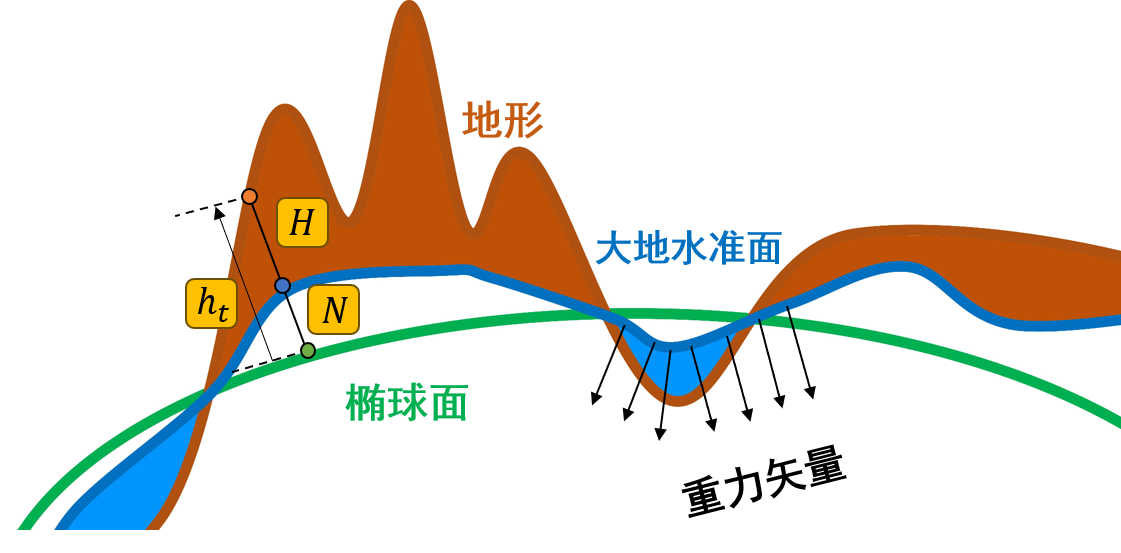
\includegraphics[width=0.9\textwidth]{figure/figure_1.png}
                  \captionsetup{font={scriptsize}}
            \end{minipage}
      }
      \subfigure[重力扰动模型]{
            \begin{minipage}{0.25\linewidth}
            \centering
                  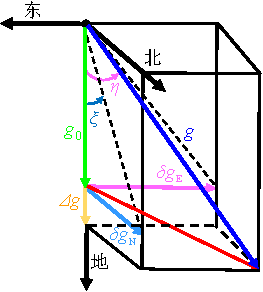
\includegraphics[width=0.9\textwidth]{figure/Mod_Gra_Dis-crop.pdf}
            \end{minipage}
      }
      \captionsetup{font={footnotesize}}
      \caption{\label{fig_1}相关模型定义}
\end{figure}

\begin{equation}
      \begin{aligned}
            \eta & \approx -\delta g_E / \gamma \\
            \xi  & \approx -\delta g_N / \gamma
      \end{aligned}
      \label{equ_1}
\end{equation}

根据几何关系可知,真实重力与正常重力、垂线偏差和重力异常之间的关系为
\begin{equation}
      \begin{aligned}
            \bm{g}^n & = \bm{\gamma}^n + \delta \bm{g}^n               \\
                     & =\begin{bmatrix}
                              0 & 0 & -\gamma
                        \end{bmatrix}^T +
            \begin{bmatrix}
                  \delta g_E & \delta g_N & \delta g_U
            \end{bmatrix}^T                       \\
                     & = \begin{bmatrix}
                               -\gamma\eta & -\gamma\xi & -\gamma - \Delta g
                         \end{bmatrix}^T
      \end{aligned}
      \label{equ_2}
\end{equation}

因此, 对于1arcsec的垂线偏差,大约会产生5mGal的水平重力误差\upcite{jekeli1994airborne},并且相关研究表明,地球海洋80\%的区域的平均垂线偏差为$5''$,15\%的区域的平均垂线偏差为$15''$,5\%的区域可达$1'$。水平方向的重力扰动分量每增加10mGal,高精度舰载惯导的位置误差约增加130m\cite{Luxin2010},而全球最大的重力扰动值可达500mGal\upcite{peshekhonov2020problem},这对于高精度惯导来说,补偿是必要的。

\section{重力扰动对惯导解算的误差影响}
黄谟涛等人提出将重力辅助惯性导航技术划分为重力补偿和重力修正两个发展阶段\upcite{WHCH20240724001},其中重力补偿技术是指在惯导解算回路中加入重力扰动信息以改善惯导系统的力学编排,达到抑制误差发散的趋势。但是,惯性导航系统的误差传播是一个动态的复杂过程,多种误差源之间(器件误差、初始条件误差、算法误差和导航环境误差)互相耦合,无法单独地分析某一变量。下面我们围绕重力扰动对惯导解算过程的影响机理进行重点分析。

\subsection{重力扰动的模型}
在惯性导航中,我们常常通过构建位置、速度和姿态误差的微分方程来描述误差源随时间传播的规律。根据上一节描述的重力扰动模型,在惯导解算的速度微分方程中,有
\begin{equation}
      \bm{\delta g^n} = \dot{\bm{v}^n}-\bm{C}^n_b\bm{f}^b+(2\bm{w}^n_{ie}+\bm{w}^n_{en})\times \bm{v}^n- \bm{\gamma}^n
      \label{equ_delta_g}
\end{equation}
在北-东-地坐标系下,可以得到其分量表示:
\begin{equation}
      \left\{ \begin{aligned}
      & \delta {{g}_{N}}={{{\dot{v}}}_{N}}-{{f}_{N}}+(2{{w}_{e}}\sin L+\frac{{{v}_{E}}\tan L}{{{R}_{N}}+h}){{v}_{E}}-\frac{{{v}_{N}}{{v}_{D}}}{{{R}_{M}}+h} \\ 
      & \delta {{g}_{E}}={{{\dot{v}}}_{E}}-{{f}_{E}}-(\frac{{{v}_{E}}}{{{R}_{N}}+h}+2{{w}_{e}}\cos L)({{v}_{D}}+{{v}_{N}}\tan L) \\ 
      & \delta {{g}_{D}}={{{\dot{v}}}_{D}}-{{f}_{D}}+\left[(2{{w}_{e}}\cos L+\frac{{{v}_{E}}}{{{R}_{N}}+h}){{v}_{E}} \right]+\frac{v_{N}^{2}}{{{R}_{M}}+h}-\gamma  \\ 
\end{aligned} \right.
\label{equ_delta_g_more}
\end{equation}
其中,$R_N$和$R_M$分别表示卯酉圈半径和子午圈半径,$L$代表纬度,$w_{e}$表示地球自转角速度,等式$\delta g_D$右边的$\left[ \cdot  \right]$为厄特弗斯效应项\upcite{harlan1968eotvos}。如果我们事先不考虑正常重力的计算误差时,那么可以将$\bm{\delta g}$视作真实的重力扰动结果。但是当我们在速度微分方程中考虑重力扰动,并将其与正常重力分开时,那么由式\ref{equ_delta_g}可以进一步得到重力扰动的误差模型,
\begin{equation}
      \begin{aligned}
      \text{d}\bm{\delta g}^n = &\bm{\delta} \dot{\bm{v}}^n + \bm{[\phi^n\times]}\bm{C}^n_b \bm{f}^b - \bm{C}^n_b \bm{\delta f}^b + 
      \\
      &(2\bm{\delta w}^n_{ie} +\bm{\delta w}^n_{en})\bm{\times v}^n+(2\bm{w}^n_{ie} + \bm{w}^n_{en})\bm{\times \delta v}^n - \bm{\delta \gamma}^n
      \end{aligned}
      \label{equ_diff_disturb}
\end{equation}
其中,$\text{d}\bm{\delta g}^n$代表重力扰动的测量误差,$\bm{[\phi^n \times]}$是姿态误差$\bm{\phi^n}$的反对称矩阵,$\bm{\delta \gamma}^n$代表正常重力的计算模型误差(当考虑惯性导航系统和卫星导航系统存在同步时间差$\text{d}T$时\upcite{schwarz1995some},式\ref{equ_diff_disturb}可以加入误差项$\ddot{\bm{v}}^n\text{d}T$)。因此,重力扰动的测量误差主要由动态加速度误差$\bm{\delta} \dot{\bm{v}}^n$、姿态误差$\bm{[\phi^n\times]}\bm{C}^n_b \bm{f}^b$和比力误差$\bm{C}^n_b \bm{\delta f}^b$引起。

\subsection{对速度的影响}
加速度计的测量误差模型为:
\begin{equation}
      \bm{\delta f}^b = \bm{b}_a + \bm{\kappa}_a \bm{f}^b + \bm{N}_a \bm{f}^b + \bm{w}_a
      \label{acc_bias}
\end{equation}
其中$\bm{b}_a$表示加速度计零偏,$\bm{\kappa}_a$为加速度计的比例因子误差矩阵,$\bm{N}_a$为交轴耦合误差矩阵,其元素表示三轴加速度计之间的非正交误差,$\bm{w}_a$表示加速度计测量值的白噪声。

当事先不考虑重力扰动时,由式\ref{equ_delta_g}可得到速度误差的微分方程,
\begin{equation}
      \begin{aligned}
      \bm{\delta \dot{v}}^n = &\bm{C}^n_b \bm{\delta f}^b - \bm{[\phi^n\times]}\bm{C}^n_b \bm{f}^b -(2\bm{w}^n_{ie} + \bm{w}^n_{en}) \times \bm{\delta v}^n \\
      &+ \bm{v}^n \times (2\bm{\delta w}^n_{ie} + \bm{\delta w}^n_{en}) + \bm{\delta g}^n
      \label{diff_delta_vel}
      \end{aligned}
\end{equation}
由\ref{diff_delta_vel}可以看出,重力扰动最直接影响的是加速度计对于速度的测量,特别体现在水平通道的上。而水平速度在经过积分计算后,最终对载体位置的解算产生影响。文献\cite{gao2021real}通过设定不同大小重力扰动的仿真试验,发现当重力扰动大于100mGal时,纯惯性导航在一天内计算的最大位置误差将超过4海里,但作者设计的仿真缺少对误差传播特性的定量分析。相反,文献\cite{WANGJING2016}将重力扰动建模为一阶马尔可夫模型,借助相关性分析,定量的确定了重力扰动引起的位置误差量级。除此之外,由于速度误差受到比力测量精度和重力扰动的共同影响,换言之,重力扰动在水平分量的速度误差传播通道与加速度计的零偏相同,故可将重力扰动等效为加速度计零偏。常路宾等人结合这个特点\upcite{chang2018gravity},具体研究了水平方向上加速度计零偏和重力扰动的关系,并结合两者之间的量级关系制定了相应的补偿策略。

\begin{figure}
      \centering
      \subfigure[北向位置误差]{
            \begin{minipage}{0.475\linewidth}
                  \centering
                  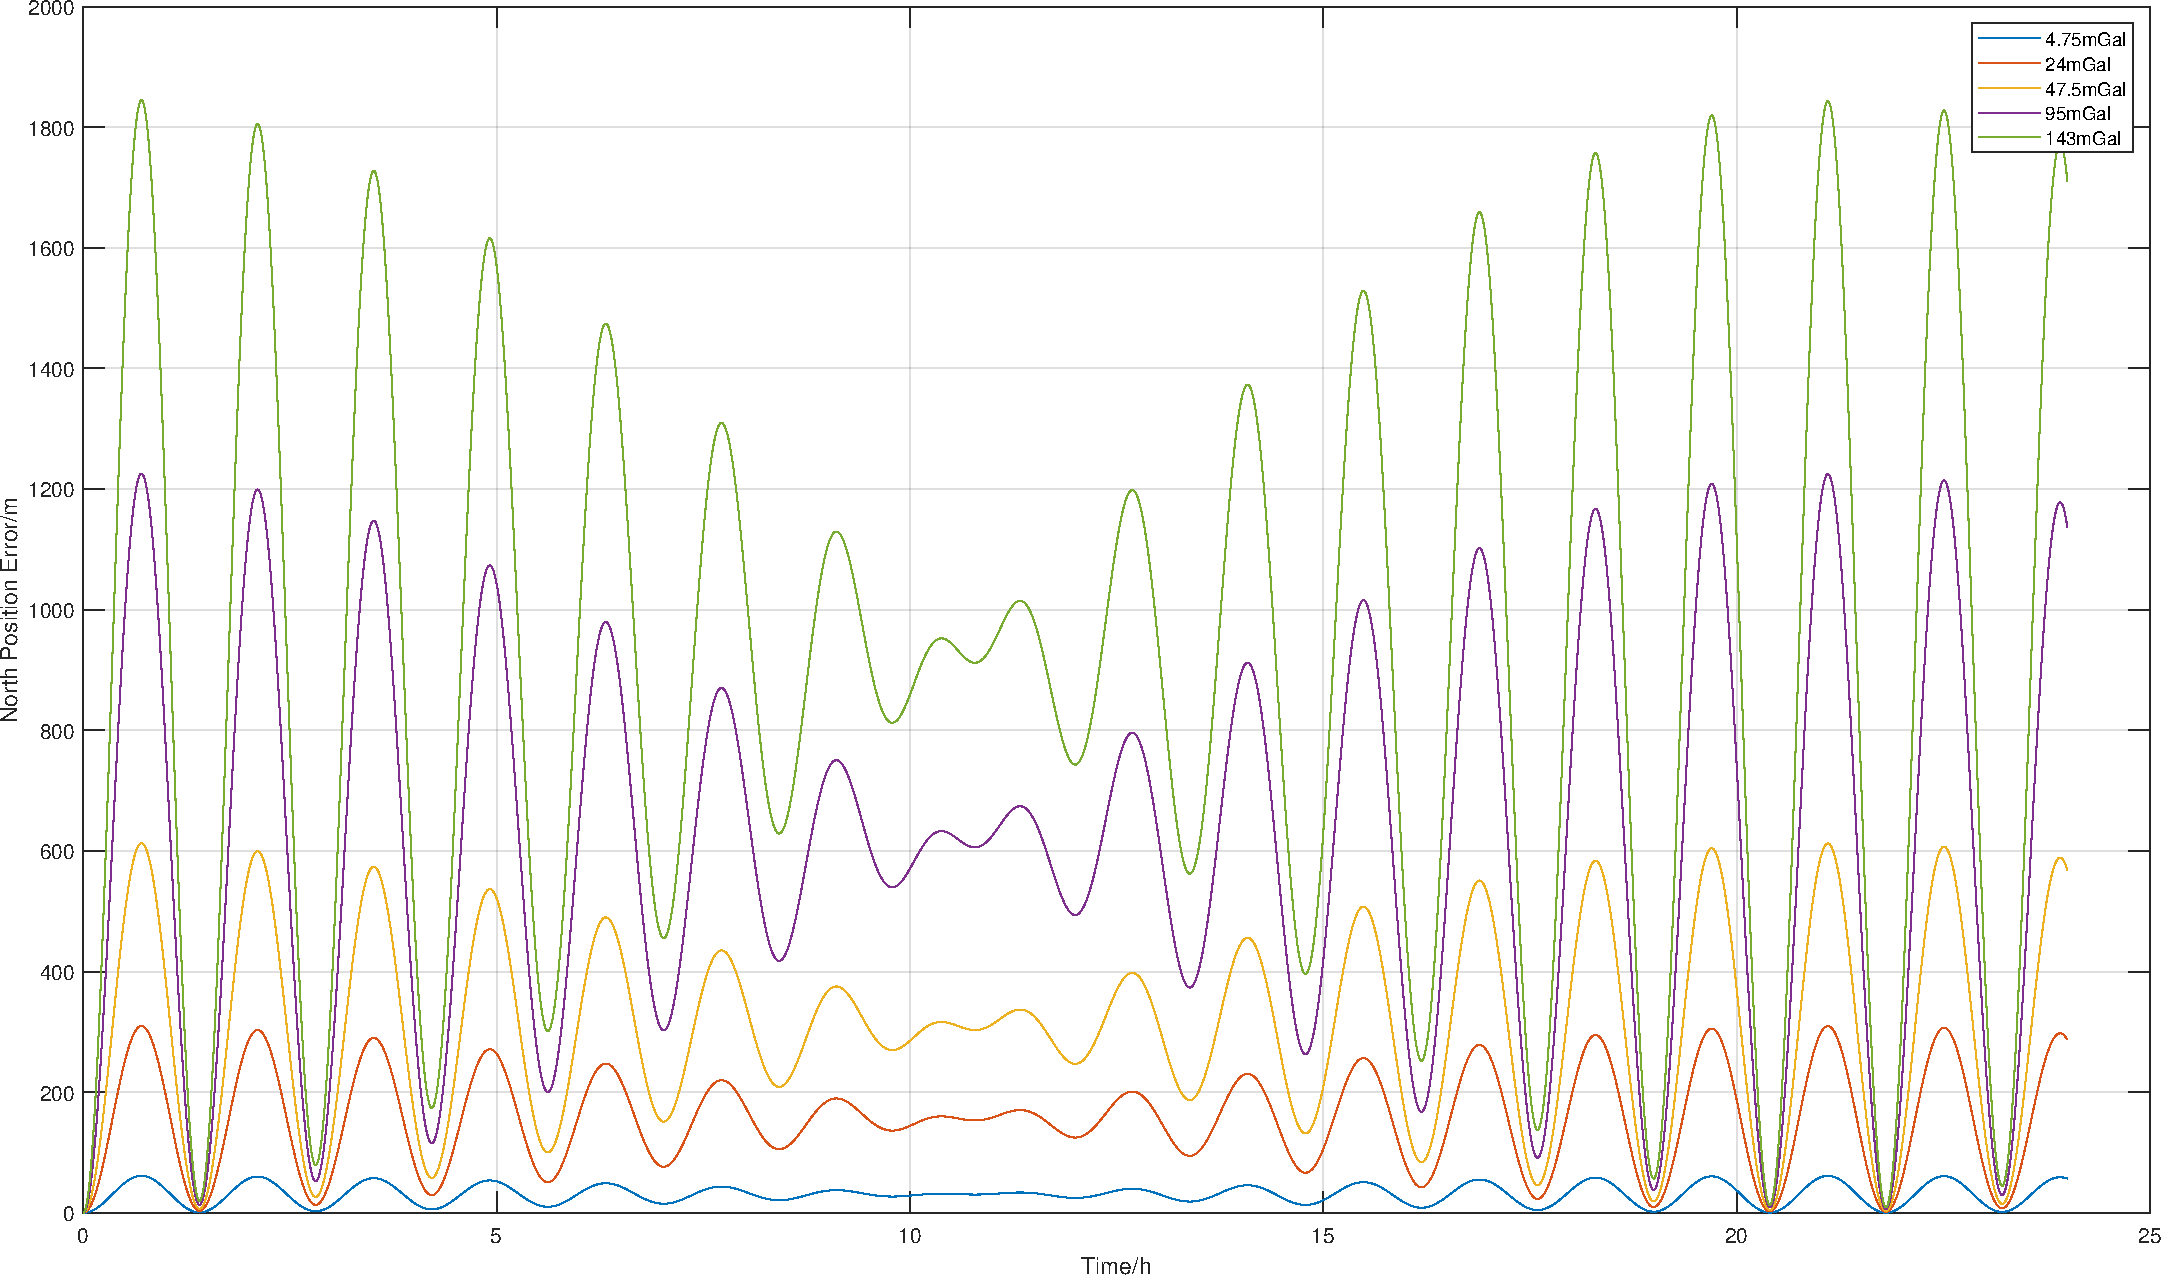
\includegraphics[width=0.99\textwidth]{figure/fig_sim_perr_nor.pdf}
            \end{minipage}
      }
      \subfigure[东向位置误差]{
            \begin{minipage}{0.475\linewidth}
            \centering
                  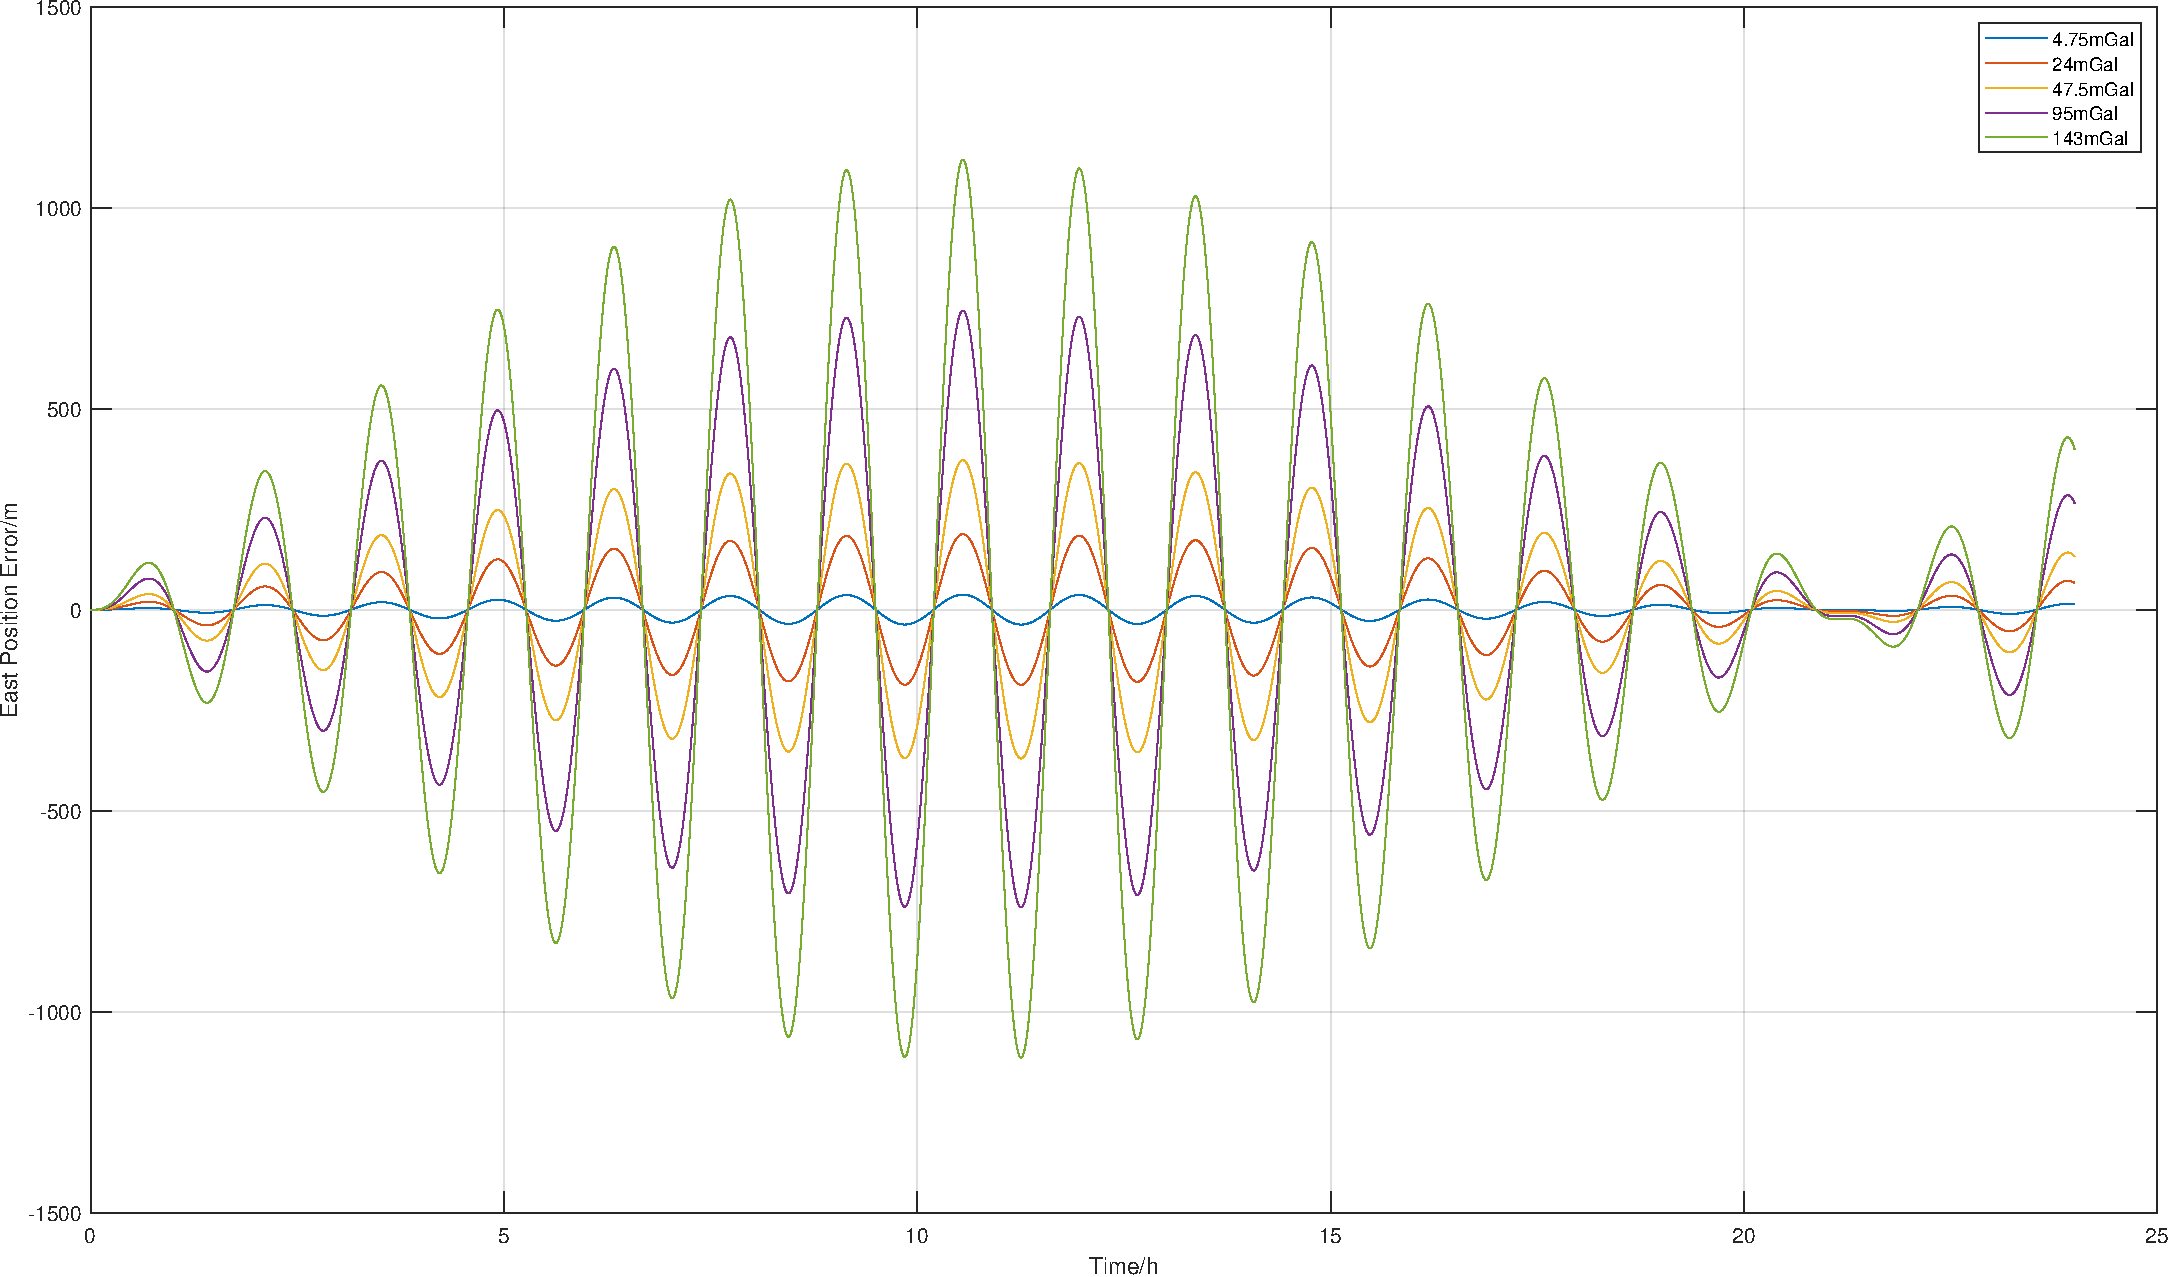
\includegraphics[width=0.99\textwidth]{figure/fig_sim_perr_eas.pdf}
            \end{minipage}
      }
      \subfigure[北向速度误差]{
            \begin{minipage}{0.475\linewidth}
                  \centering
                  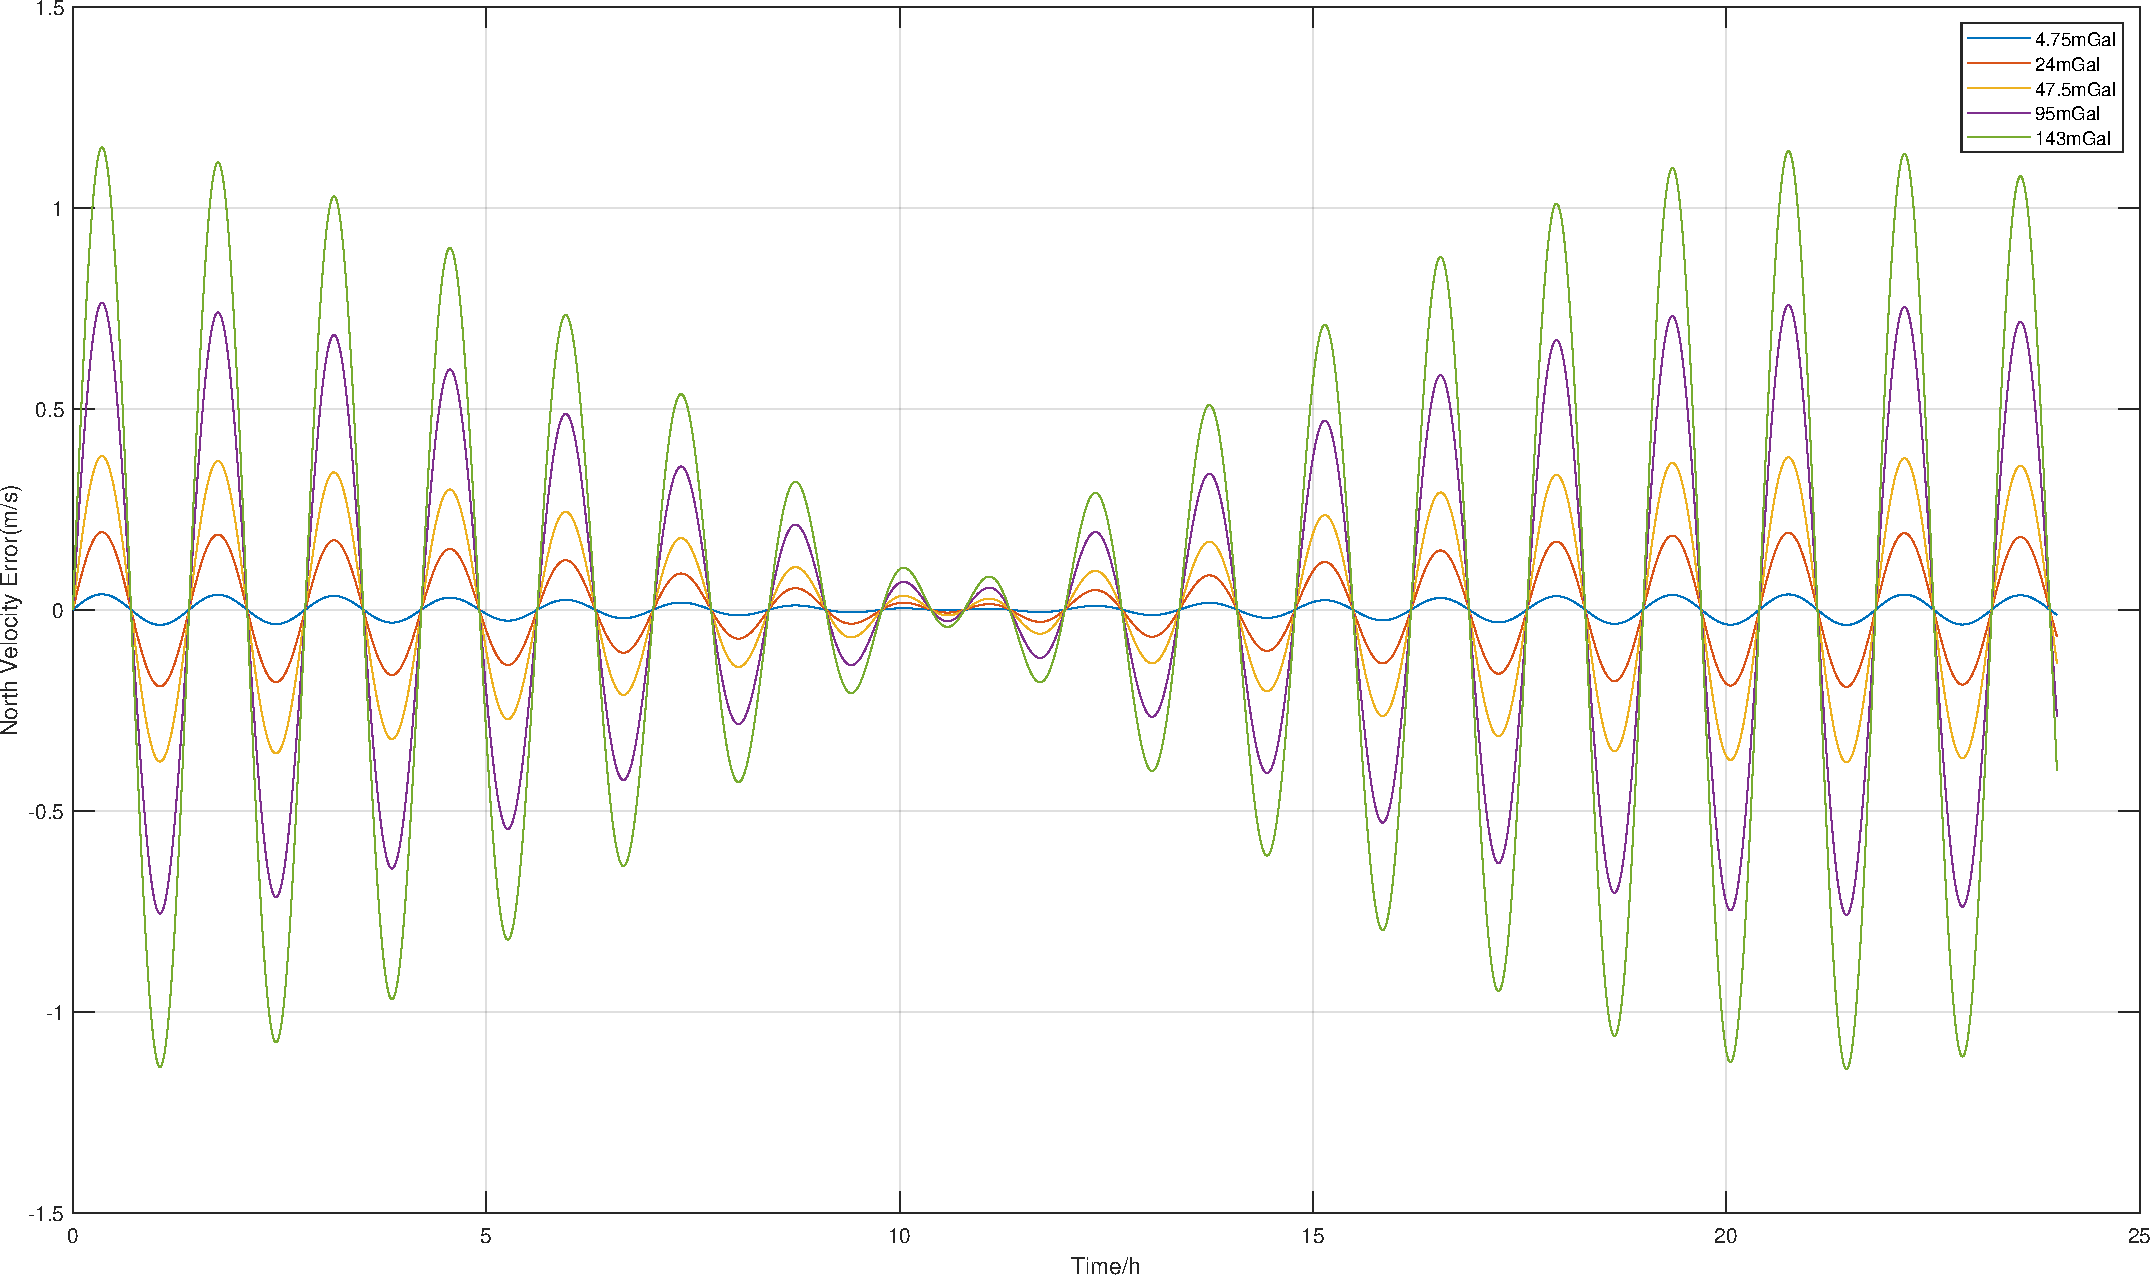
\includegraphics[width=0.99\textwidth]{figure/fig_sim_verr_nor.pdf}
                  \captionsetup{font={scriptsize}}
            \end{minipage}
      }
      \subfigure[东向速度误差]{
            \begin{minipage}{0.475\linewidth}
            \centering
                  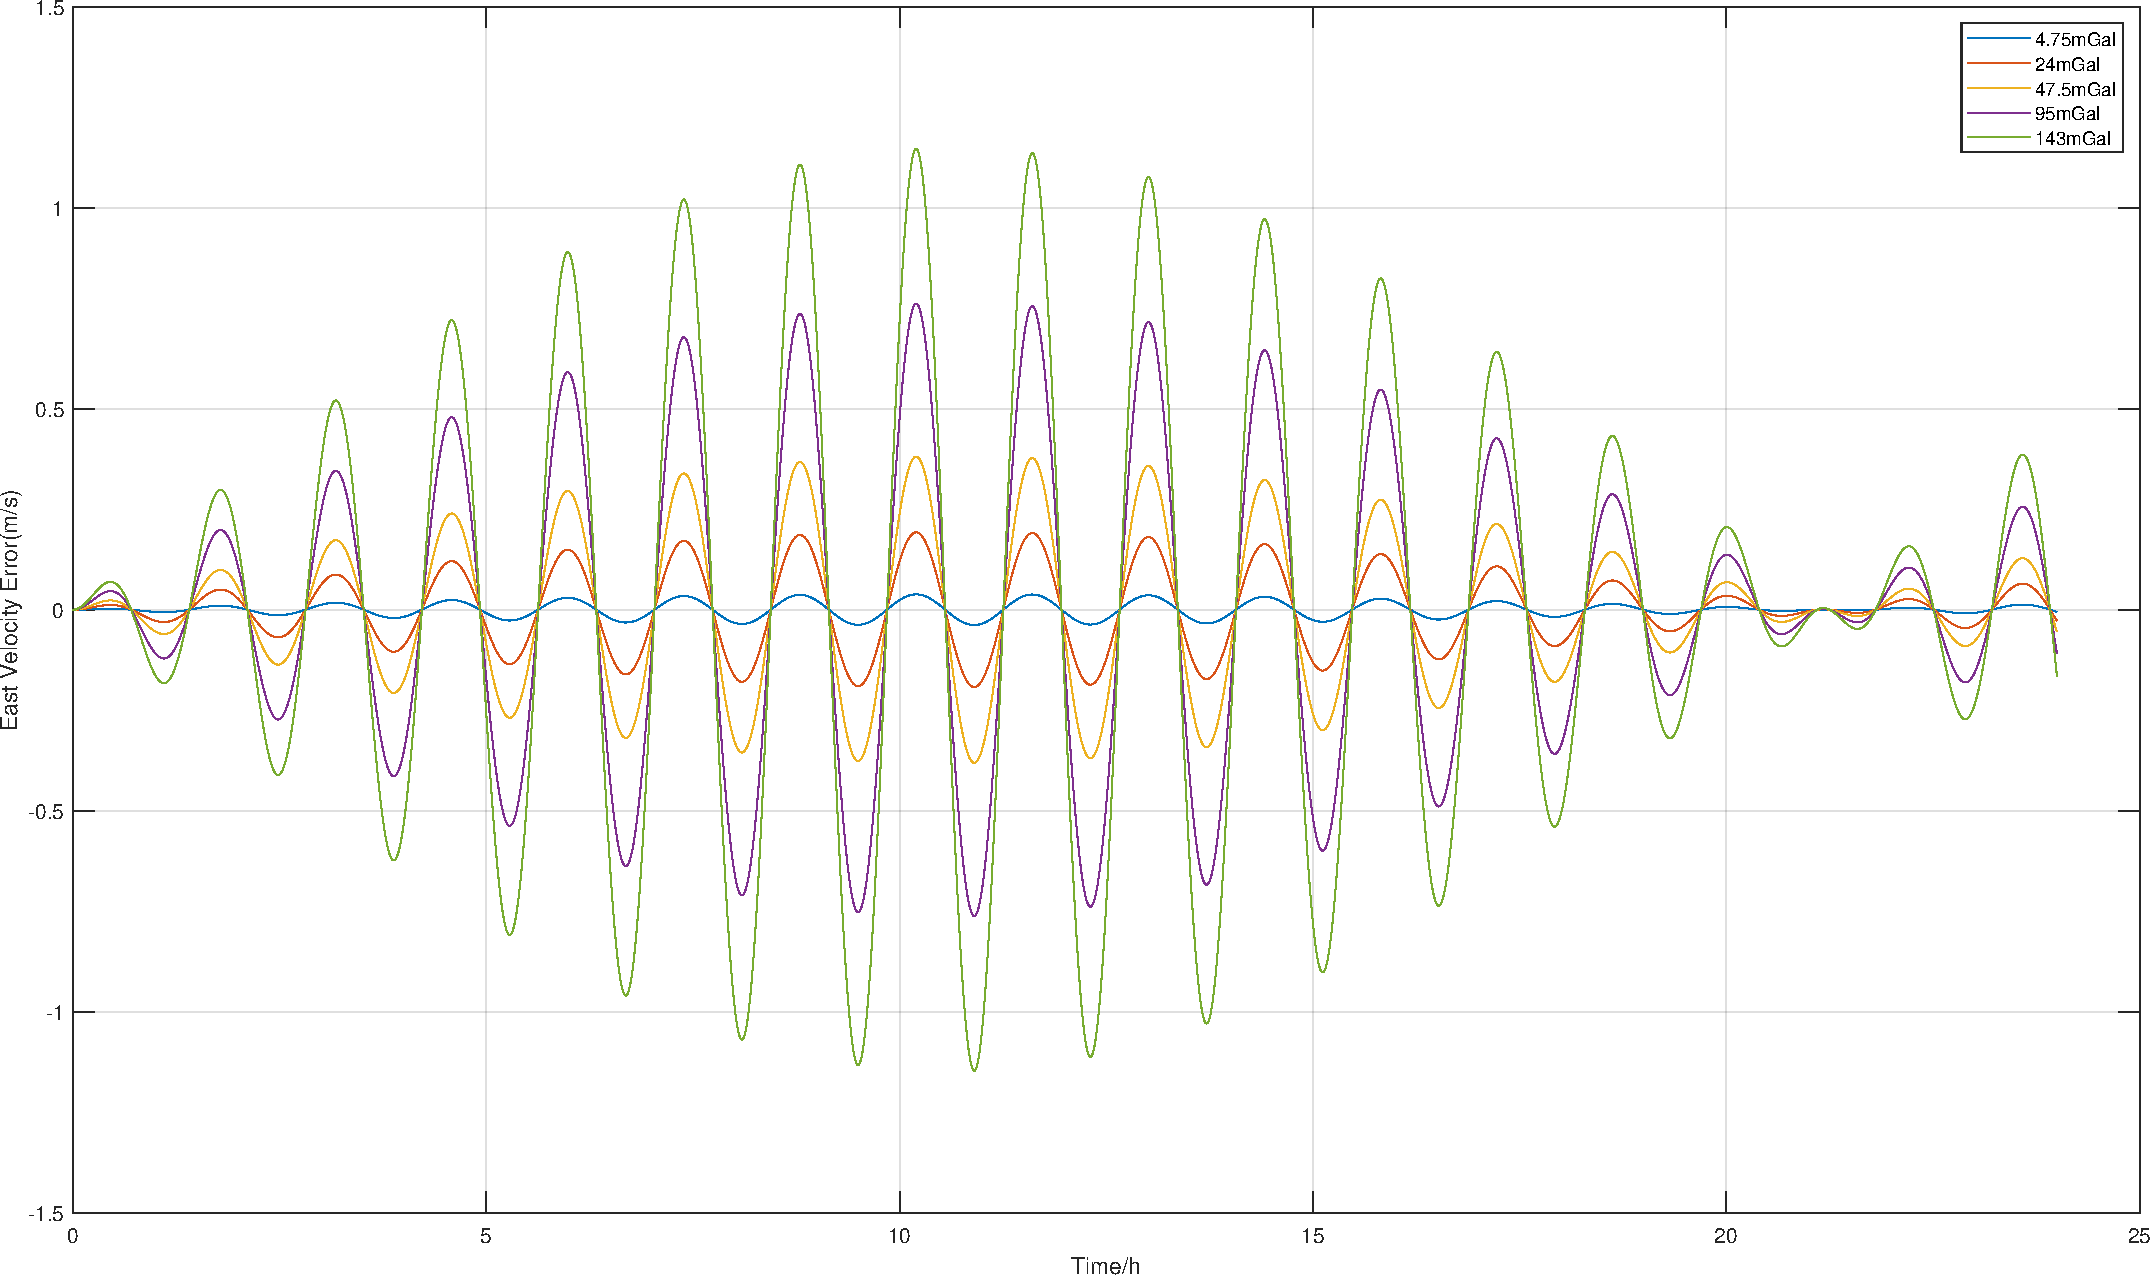
\includegraphics[width=0.99\textwidth]{figure/fig_sim_verr_eas.pdf}
            \end{minipage}
      }
      \captionsetup{font={footnotesize}}
      \caption{\label{fig:sim_gra_dis_nor}北向重力扰动的仿真实验}
\end{figure}

% \begin{figure}
%       \centering
%       \subfigure[北向位置误差]{
%             \begin{minipage}{0.47\linewidth}
%                   \centering
%                   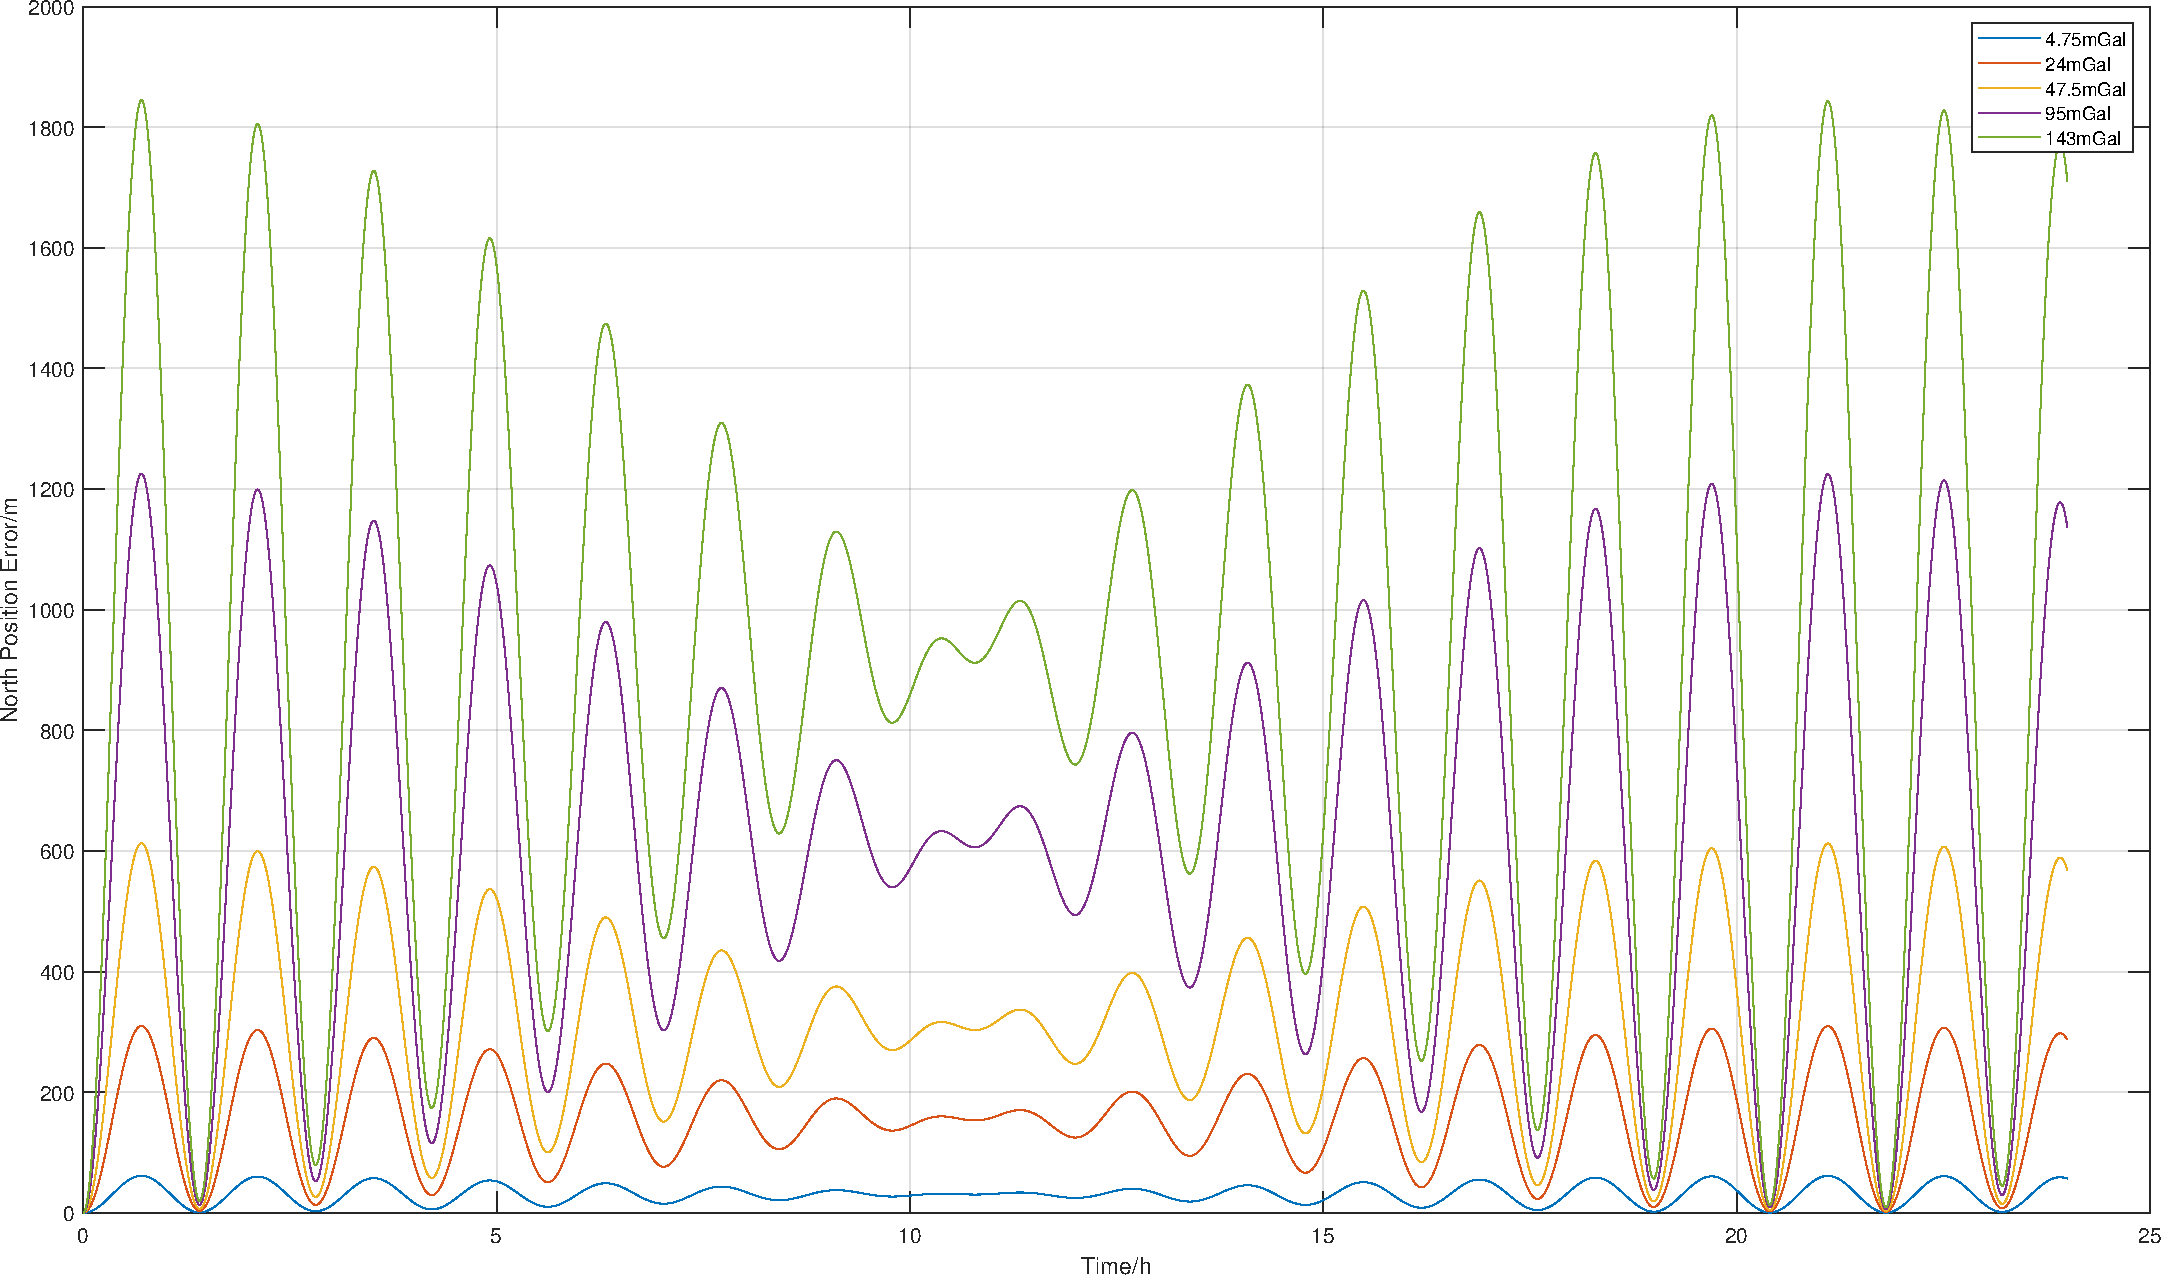
\includegraphics[width=0.9\textwidth]{figure/fig_sim_perr_nor.pdf}
%             \end{minipage}
%       }
      
%       \subfigure[东向位置误差]{
%             \begin{minipage}{0.47\linewidth}
%             \centering
%                   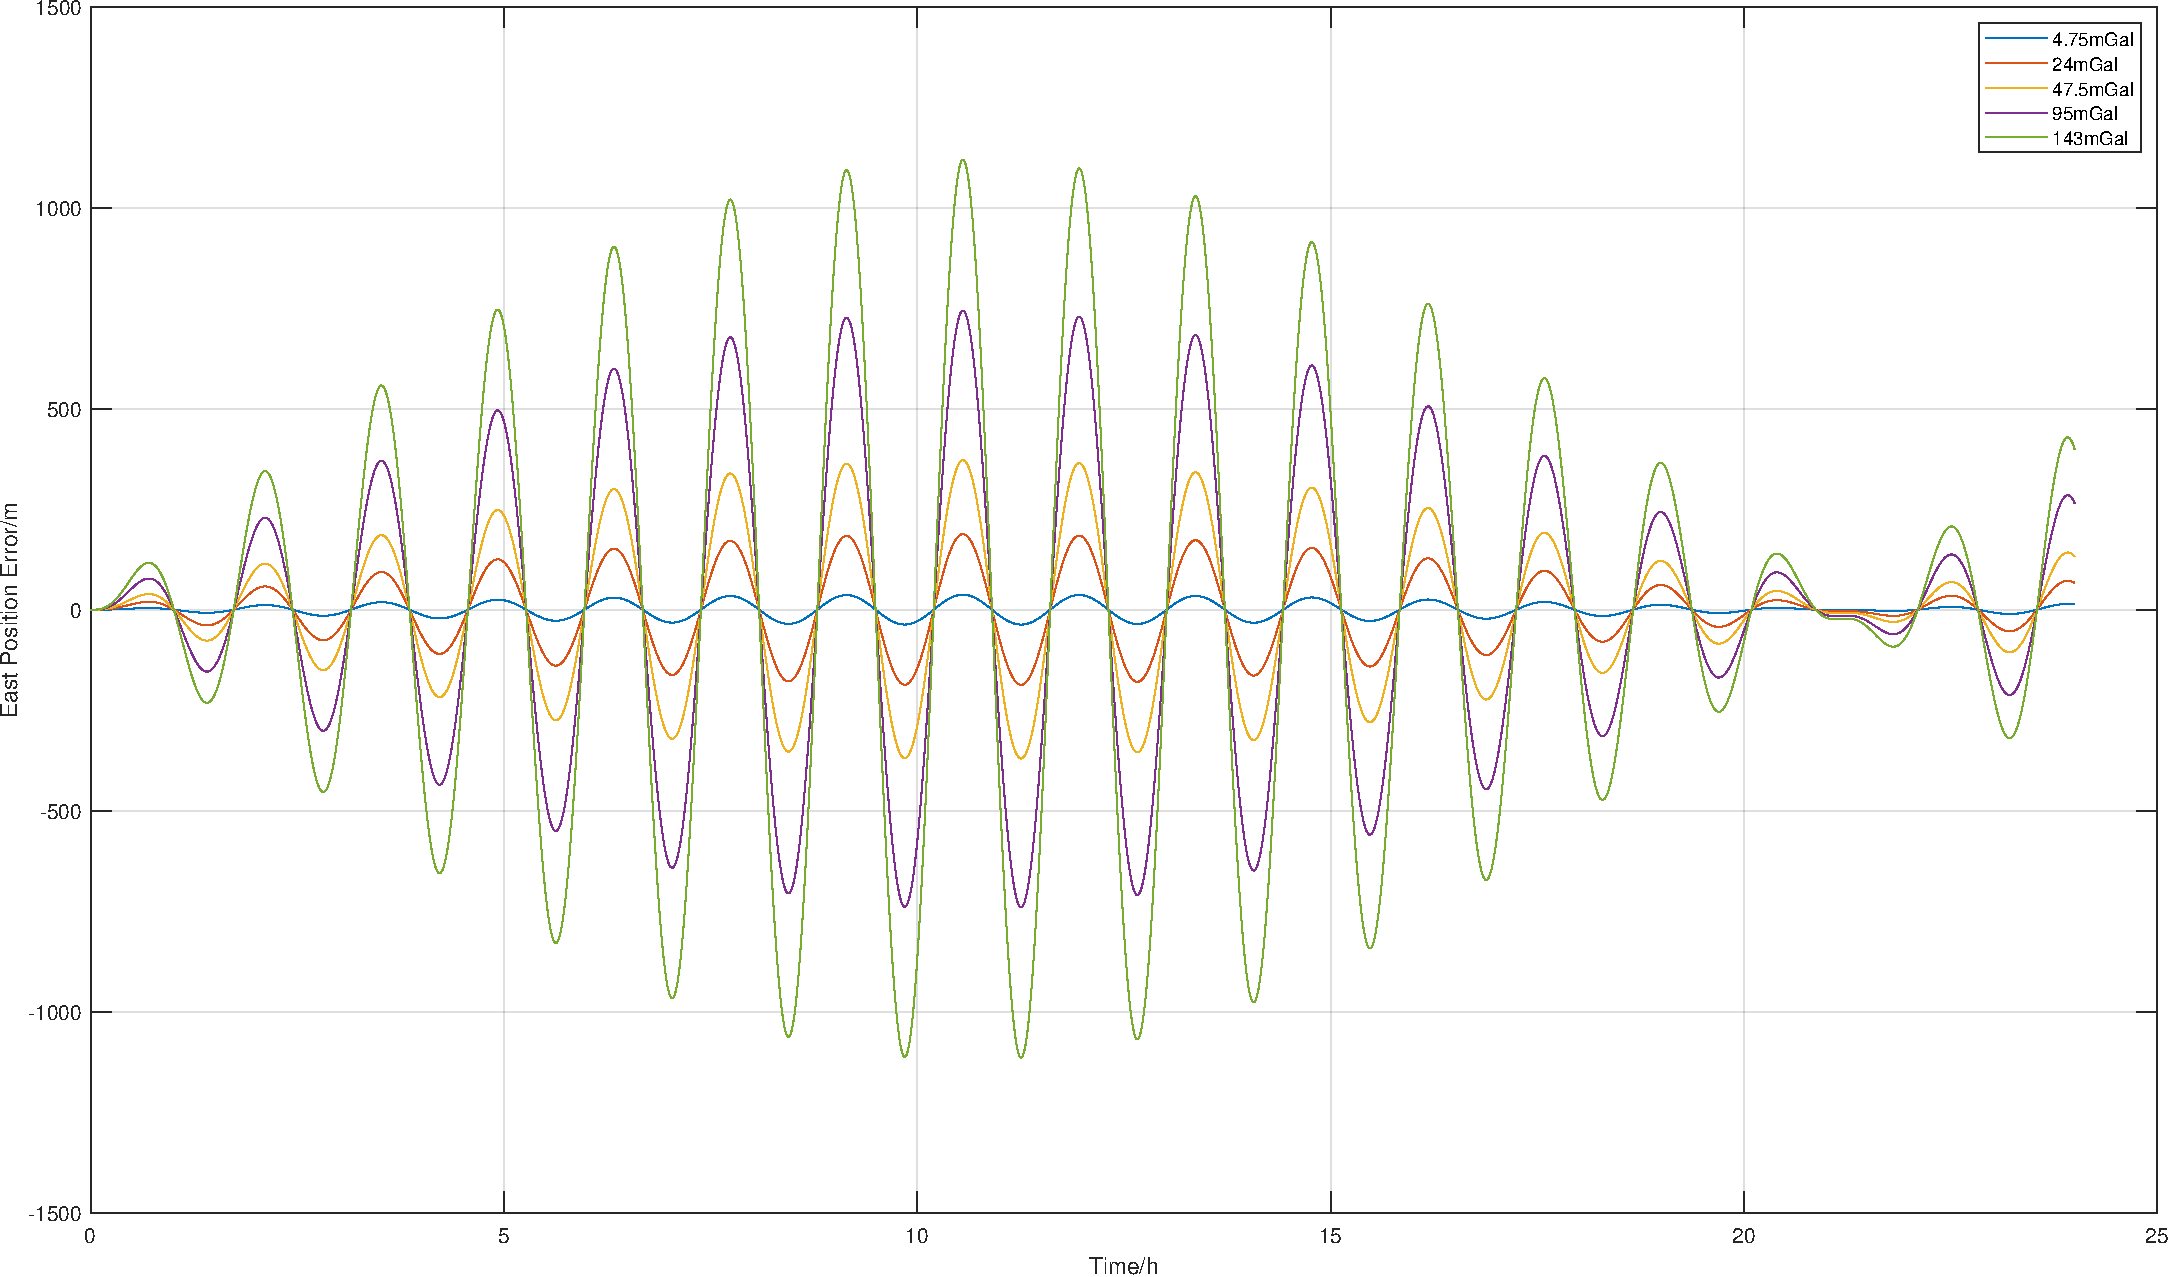
\includegraphics[width=0.9\textwidth]{figure/fig_sim_perr_eas.pdf}
%             \end{minipage}
%       }

%       \subfigure[北向速度误差]{
%             \begin{minipage}{0.47\linewidth}
%                   \centering
%                   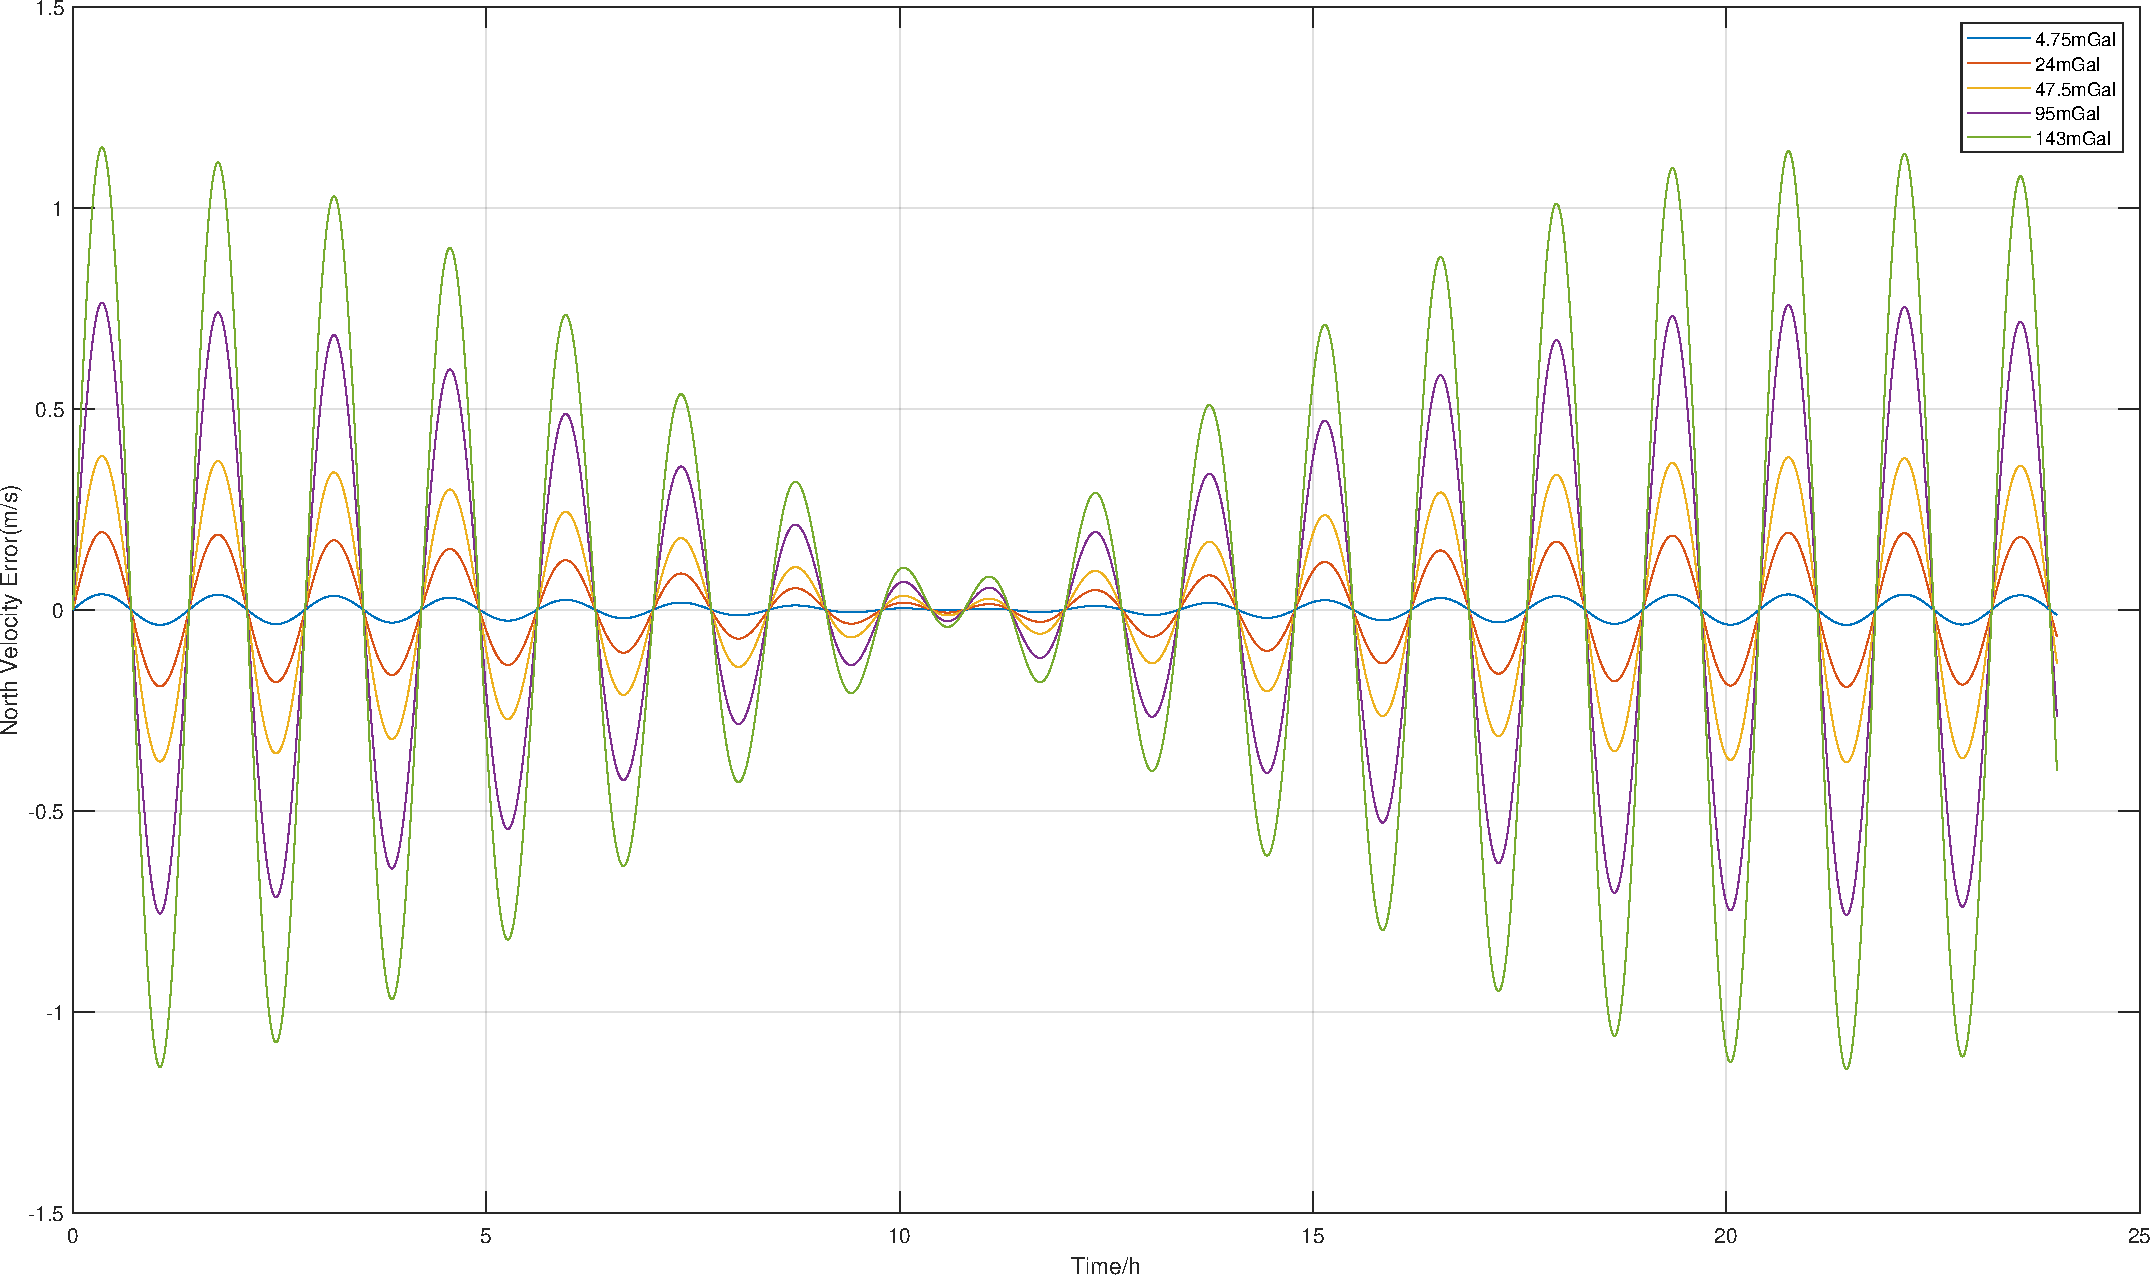
\includegraphics[width=0.9\textwidth]{figure/fig_sim_verr_nor.pdf}
%                   \captionsetup{font={scriptsize}}
%             \end{minipage}
%       }

%       \subfigure[东向速度误差]{
%             \begin{minipage}{0.47\linewidth}
%             \centering
%                   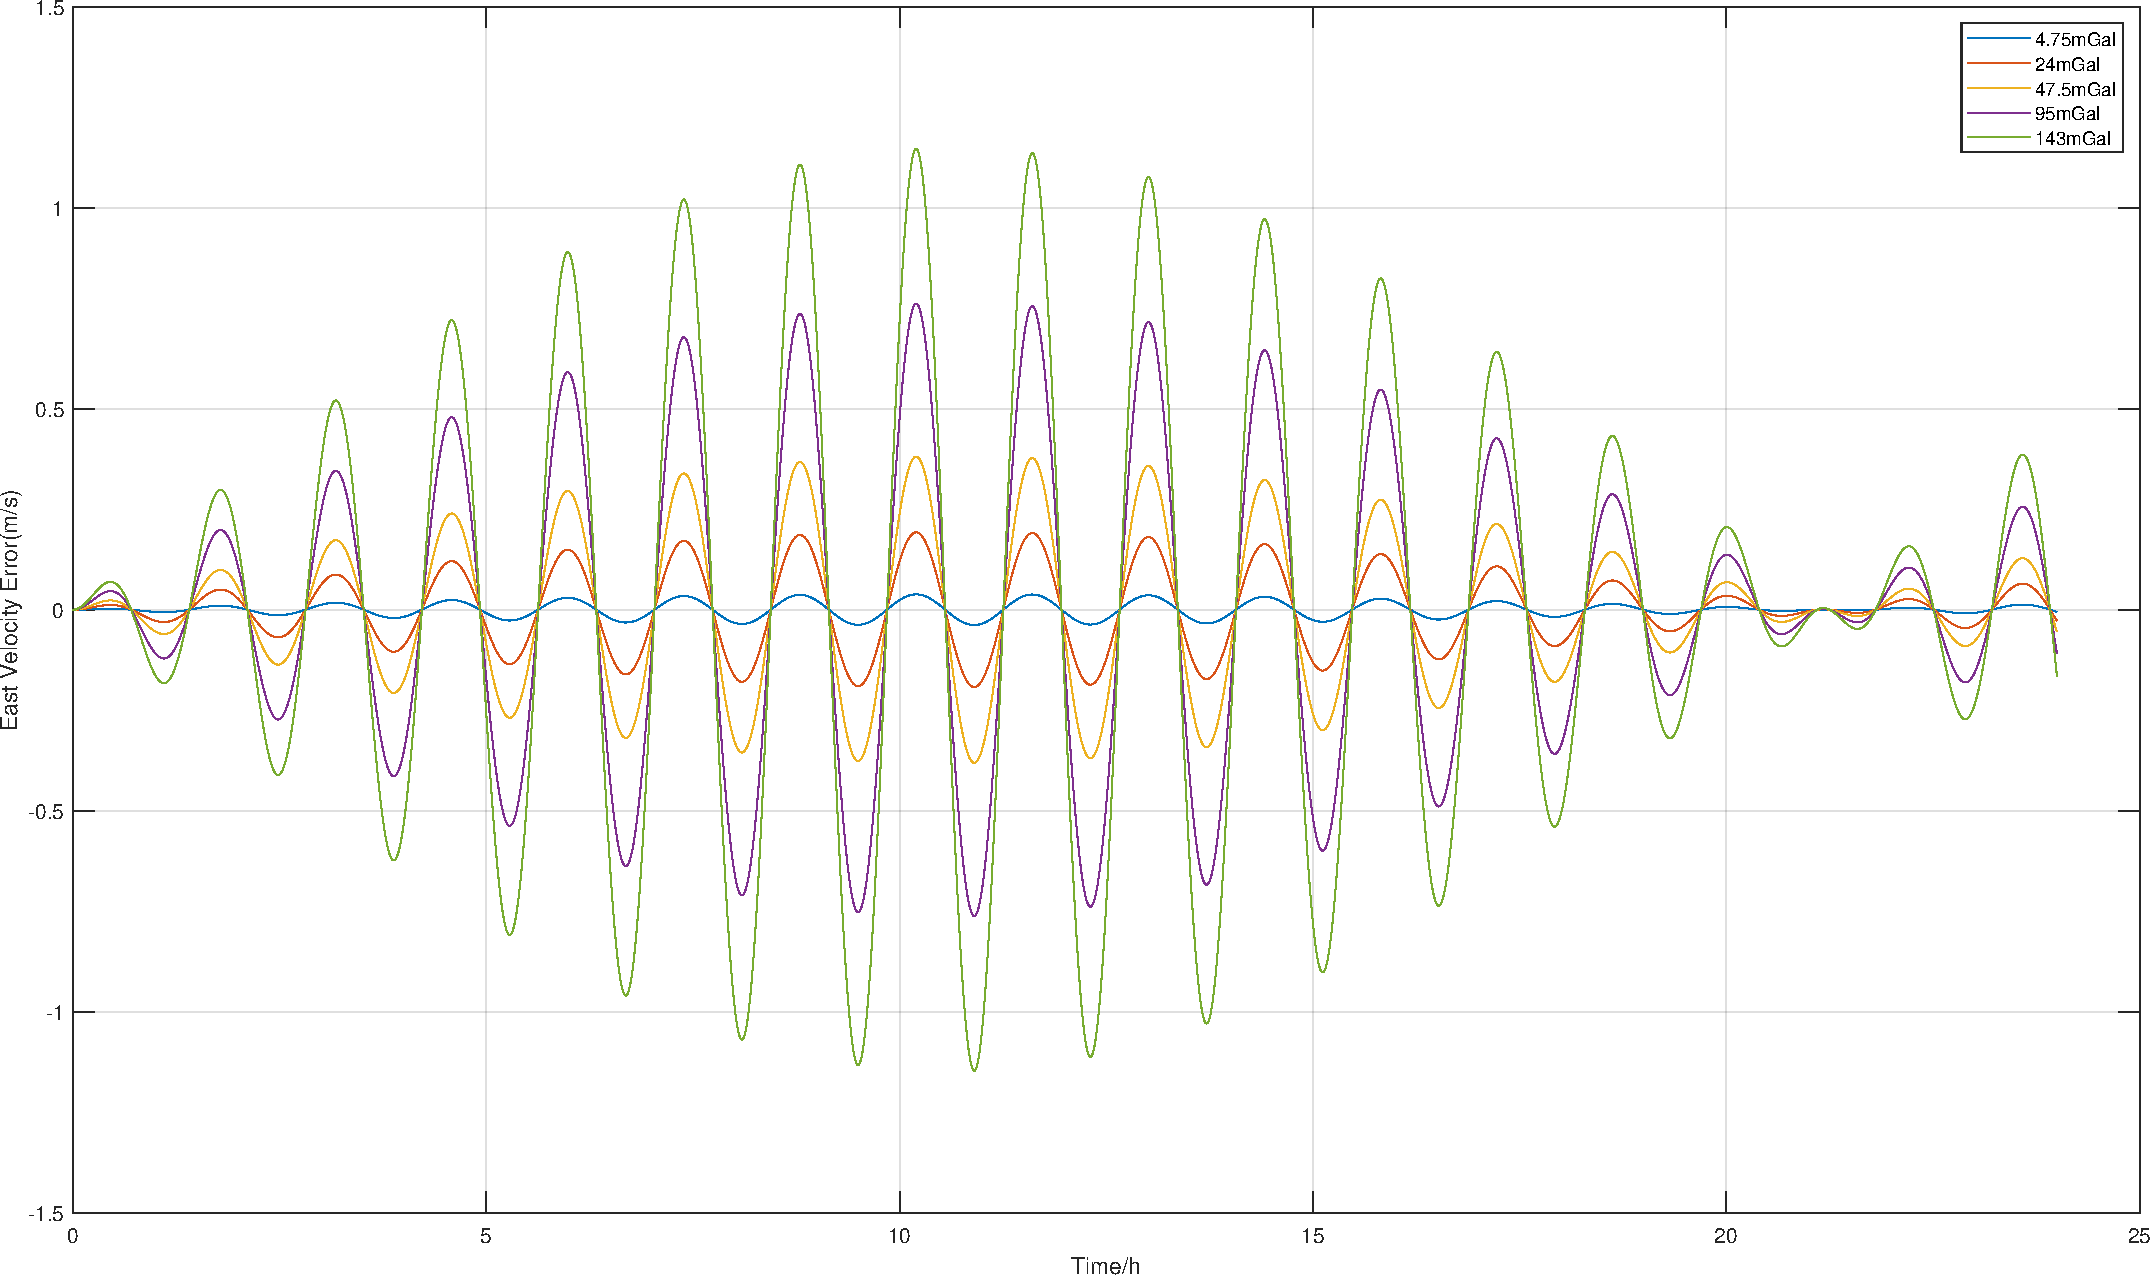
\includegraphics[width=0.9\textwidth]{figure/fig_sim_verr_eas.pdf}
%             \end{minipage}
%       }
%       \captionsetup{font={footnotesize}}
%       \caption{\label{fig:sim_gra_dis_nor}北向重力扰动的仿真实验}
% \end{figure}

\subsection{对姿态的影响}
% 惯导的姿态误差可以通过式 来表示,
% \begin{equation}
%       \bm{\phi}^n = \bm{\phi}^n_0 + \int_{t_0}^{t}{\bm{C}^n_b \,\text{d}w^b_{ib} \,\text{d}t}
% \end{equation}
% 其中第一项$\bm{\phi}^n_0$代表初始对准误差,包括重力异常误差;第二项主要是陀螺自身引起的器件误差,包括陀螺轴非正交误差,比例因子误差,线性和非线性漂移,随机游走,量化噪声和分形噪声等\upcite{savage1978strapdown,li1995chaotic}。
在与GNSS集成的捷联惯导系统中,理论和实验证明,垂线偏差的引入会带来倾斜误差,因此需要进行垂线偏差补偿以提高姿态精度\upcite{grejner1998gravity,dai2015dynamic}。
陀螺的测量误差模型为:
\begin{equation}
      \bm{\delta w}^b_{ib} = \bm{b}_g + \bm{\kappa}_g \bm{ w}^b_{ib} + \bm{N}_g \bm{ w}^b_{ib} + \bm{w}_g
      \label{gyro_bias}
\end{equation}
将惯导解算中的姿态误差微分方程展开,如式子\ref{equ_phi_more}所示
\begin{equation}
            \left\{ \begin{aligned}
            & \dot{\bm{\phi}}_N=-\frac{w_e\sin L}{R_M + h}\delta r_N+\frac{v_E}{(R_N+h)^2}\delta r_D + \frac{1}{R_N + h}\delta v_E \\
            & \ \ \ \ \ \ \ \ - \left ( w_e\sin L + \frac{v_E\tan L}{R_N +h} \right )\phi_E + \frac{v_N}{R_M+h}\phi_D - \delta w^n_{ib,N} \\ 
            & \dot{\bm{\phi}}_E= - \frac{v_N}{(R_M + h)^2}\delta r_D - \frac{1}{R_M + h }\delta v_N \\
            & \ \ \ \ \ \ \ \ + \left ( w_e \sin L + \frac{v_E\tan L}{R_N + h} \right )\phi_N + \left ( w_e \cos L +\frac{v_E}{R_N + h} \right )\phi_D - \delta w^n_{ib,E}\\ 
            & \dot{\bm{\phi}}_D= - \left [ \frac{w_e\cos L}{R_M + h}+ \frac{v_E\sec ^2L}{(R_M + h)(R_N + h)}\right ]\delta r_N - \frac{v_E \tan L}{(R_N+h)^2}\delta r_D - \frac{\tan L}{R_N + h}\delta v_E \\
            & \ \ \ \ \ \ \ \ - \frac{v_N}{R_M + h}\phi_N - \left ( w_e \cos L + \frac{v_E}{R_N + h } \right )\phi_E - \delta w^n_{ib,D}
      \end{aligned} \right.
      \label{equ_phi_more}
\end{equation}

\begin{figure}[h]
      \centering
      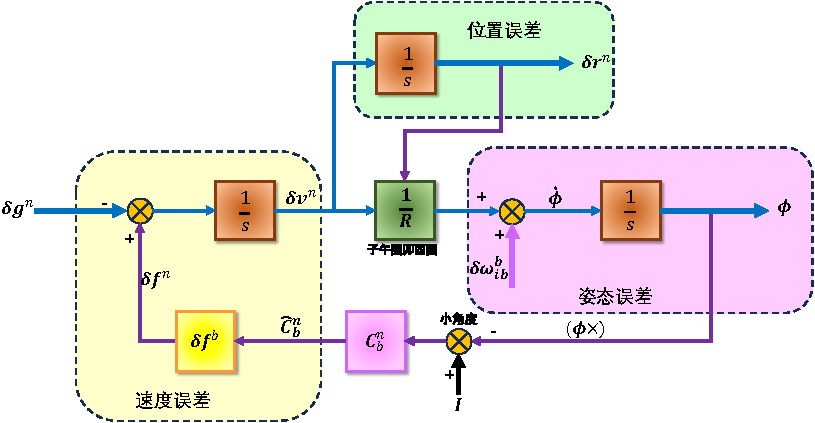
\includegraphics[width=0.65\textwidth]{figure/fig_error_sep-crop.pdf}
      \captionsetup{font={footnotesize}}
      \caption{\label{fig:error_sep}重力扰动的误差传播途径}
\end{figure}

虽然姿态误差微分方程中没有直接体现重力扰动的表达式,但是结合前面重力扰动对速度误差的分析可以知道,重力扰动通过影响速度误差进而影响位置误差,最终二者共同影响姿态误差。图\ref{fig:error_sep}为重力扰动对速度误差、位置误差和姿态误差的传播路径示意图,首先重力扰动会与加速度计器件误差一起耦合,在第一次对时间积分下形成速度误差,接着速度误差继续积分得到位置误差,而根据式\ref{equ_phi_more}速度误差和位置误差会与陀螺器件误差一起形成角加速度误差,在积分后会形成姿态角误差,而姿态角误差会导致载体系与导航系产生旋转偏差,进而影响到加速度计的输出结果。

此外,相关研究表明\upcite{jekeli1994airborne,1020386196.nh,harriman1986gravity,Zhangpanpan23},当载体运动时,如果速度较大,姿态误差则主要由水平重力扰动的中低频分量(波长$\lambda_0>30$km)引起;随着载体速度减小,高频分量则占主导地位,换句话说,低速运动的载体所经历的重力场细节特征作用更加明显,对姿态误差影响更大,因此确定水平重力扰动的高频信号是进一步提高重力补偿精度的关键。

\subsection{对初始对准的影响}
在惯导系统进行初始对准时期,在初始条件$v_D =v_E=0, \dot{v}_D=\dot{v}_E = 0, f_D = f_E = 0, f_U = \gamma$下,如果我们事先并不考虑重力扰动项\upcite{LUOKAIXIN2023},而视作重力模型误差,将其带入速度误差微方程,可以得到
\begin{equation}
      \left\{ \begin{aligned}
            &\delta \dot{v}_N = -f_D\phi_E + \delta g_N + \delta f_N
            \\
            &\delta \dot{v}_E = f_D\phi_N + \delta g_E + \delta f_E
      \end{aligned} \right.
\end{equation}
于是,北向和东向姿态角误差可以写作
\begin{equation}
      \left\{ \begin{aligned}
            &\phi_N = \frac{\delta \dot{v}_E - \delta f_E - \delta g_E}{\gamma} =  \eta - \frac{\delta f_E}{\gamma}
            \\
            &\phi_E = \frac{-\delta \dot{v}_N + \delta g_N + \delta f_N}{\gamma} = -\xi + \frac{\delta f_N}{\gamma}
      \end{aligned} \right.
      \label{equ_phi_align}
\end{equation}
而根据姿态角误差微分方程\ref{equ_phi_more}可以得到
\begin{equation}
      \left\{ \begin{aligned}
      & \dot{\bm{\phi}}_N=-\phi_E w_e\sin L - \delta w^n_{ib,N} 
      \\ 
      & \dot{\bm{\phi}}_E= \phi_N w_e \sin L + \phi_D w_e \cos L - \delta w^n_{ib,E}
      \\ 
      & \dot{\bm{\phi}}_D = -\phi_E w_e \cos L - \delta w^n_{ib,D}
\end{aligned} \right.
\label{equ_phi_delta_align}
\end{equation}
结合式\ref{equ_phi_delta_align}中第二项,并将\ref{equ_phi_align}代入求解,得到
\begin{equation}
      \begin{aligned}
      \phi_D &= \frac{\dot{\phi}_E - \phi_N w_e \sin L +\delta w^n_{ib,E}}{w_e\cos L}
      \\
      &= \frac{-\dot{\xi} + \frac{\delta \dot{f}_N}{\gamma}}{w_e\cos L} - (\eta - \frac{\delta f_E}{\gamma})\tan L + \frac{\delta w^n_{ib,E}}{w_e\cos L}
      \end{aligned}
\end{equation}
而当我们通过滤波等其它方法得到收敛的$\dot{\xi}$和$ \delta \dot{f}_N$结果时\upcite{soler2014deflection},最终可以得到
\begin{equation}
      \phi_D = -(\eta - \frac{\delta f_E}{\gamma})\tan L + \frac{\delta w^n_{ib,E}}{w_e\cos L}
\end{equation}

综上所述,在初始对准时,北向姿态角误差和地向姿态角误差会与东向垂线偏差有关,东向姿态角误差与北向垂线偏差有关。
% 我们往往采用的是模型计算得到的正常重力,而又由第三节可知,参与惯导解算的正常重力和真实重力之间存在着垂线偏差,这就导致初始对准解算得到的姿态结果含有误差,从而产生惯导解算误差\upcite{LUOKAIXIN2023}。

为了分析重力扰动对初始对准过程的影响,朱靖基于海洋重力场信息与激光陀螺姿态测量系统(Attitude $\And$ Heading Measurement System, AHMS)\upcite{1020386196.nh},针对在不同工作模式下DOV对初始对准精度的影响进行了分析和仿真验证,结果表明,单轴旋转系统的对准精度随DOV增大而降低,随着对准时间的增加,引起的姿态误差趋于计算的理论值。同样的,文献\cite{hao2022analysis}结合单轴旋转惯导的旋转调制方法,对初始对准过程中的姿态误差进行了精细对准,并推导出了考虑IMU和DOV耦合的理论极限误差方程。在此基础之上,张盼盼进一步地借助双轴旋转惯导的优势\upcite{zhang2023gravity},将加速度计的漂移进行准确的估计后,通过静态仿真实验验证了重力扰动对北向和东向姿态误差的影响,并通过补偿重力扰动,成功减小了姿态误差。但是相反,文献\cite{TIE2017impact}使用EGM2008模型在初始对准过程进行重力扰动补偿后,得到的惯导精度反而更差。可能存在的原因是,作者在试验过程中没有厘清加速度计零偏和重力扰动的耦合关系,所以对重力扰动进行补偿后相当于引入了额外的误差。不拘泥于传统的对准方法,文献\cite{hao2022relative}提出了基于双重对准的相对估计方法,通过在INS中进行双重对准和姿态跟踪,提高了垂线偏差估计的精度和效率。但是该方法由于关注于DOV的估计,对于系统中的其他误差源的影响可能并没有充分考虑。文献\cite{tie2018compensation}根据重力扰动会导致对准坐标系与导航坐标系不一致的结果,提出了基于惯导解算过程中的速度和姿态的两种补偿方法,对于船舶导航实验,其定位精度提高了10\%左右。与初始对准情况类似,当不存在外部观测的情况下,使用零速修正(Zero velocity update,ZUPT)对于惯导误差的发散过程有一定的约束作用,文献\cite{Wumingqiang2023}\cite{weng2020analysis}则研究了重力扰动对零速修正方法的影响,并采取了常用的补偿策略提高了位置精度。

\section{现有的补偿方法}
\subsection{基于球谐模型补偿}
上个世纪70年代起,越来越多的卫星用于重力场的重建,其中GEM(Goddard Earth Model)和TEG(Texas Earth Gravity models)模型开发团队在联合重力建模工作上取得了重大进展\upcite{lerch1972gravitational,tapley1997teg},但是构建海洋重力场模型的不确定因素在于目前对海洋地形的模拟不足,即海面与大地水准面之间的高度差,而基于测高的海洋大地水准面和重力场模型是计算组合重力场模型的重要数据源\upcite{pavlis2012development,flechtner2021satellite}。目前国际上可以准确估计重力场信息的公开球谐函数模型有美国国家地理空间情报局(National Geospatial-Intelligence Agency, NGA)发布的EGM2008和由德国波茨坦地球科学研究中心German Research Centre for Geosciences(GFZ Potsdam)发布的EIGEN-6C4,图\ref{fig:model_ICGEM}所示为EIGEN-6C4模型与EGM2008模型的相关计算结果。
\begin{figure}
      \centering
      \subfigure[EIGEN-6C4模型与EGM2008模型重力异常差值]{
            \begin{minipage}{0.507\linewidth}
                  \centering
                  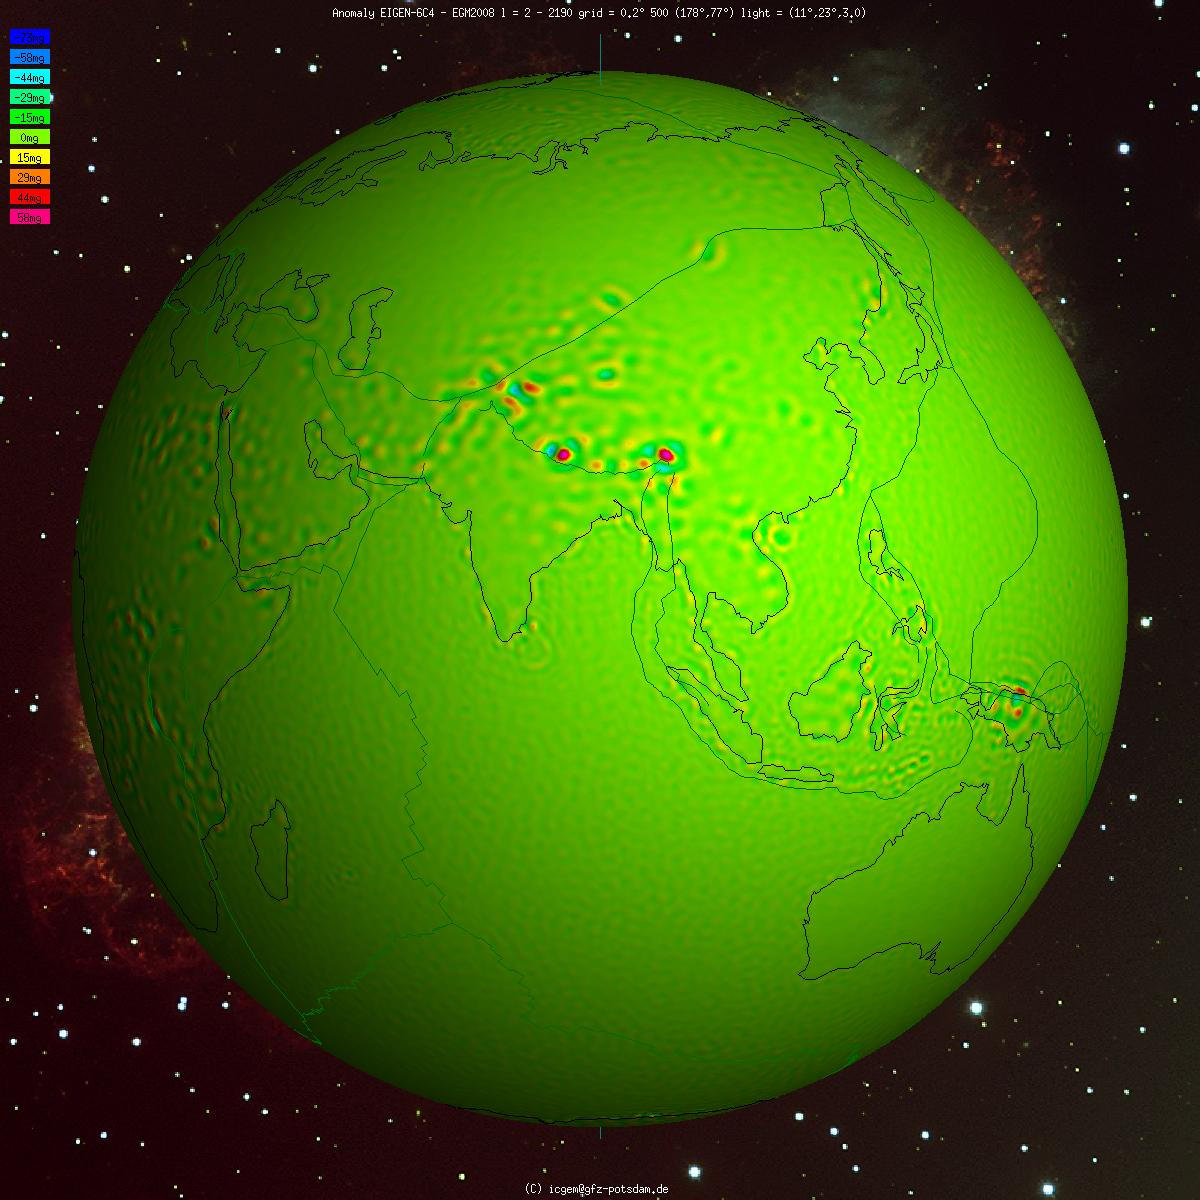
\includegraphics[width=0.83\textwidth]{figure/differ_anomaly_eigen-6c4toegm2008.jpg}
                  \captionsetup{font={scriptsize}}
            \end{minipage}
      }
      \subfigure[EIGEN-6C4重力扰动网格计算结果]{
            \begin{minipage}{0.449\linewidth}
            \centering
                  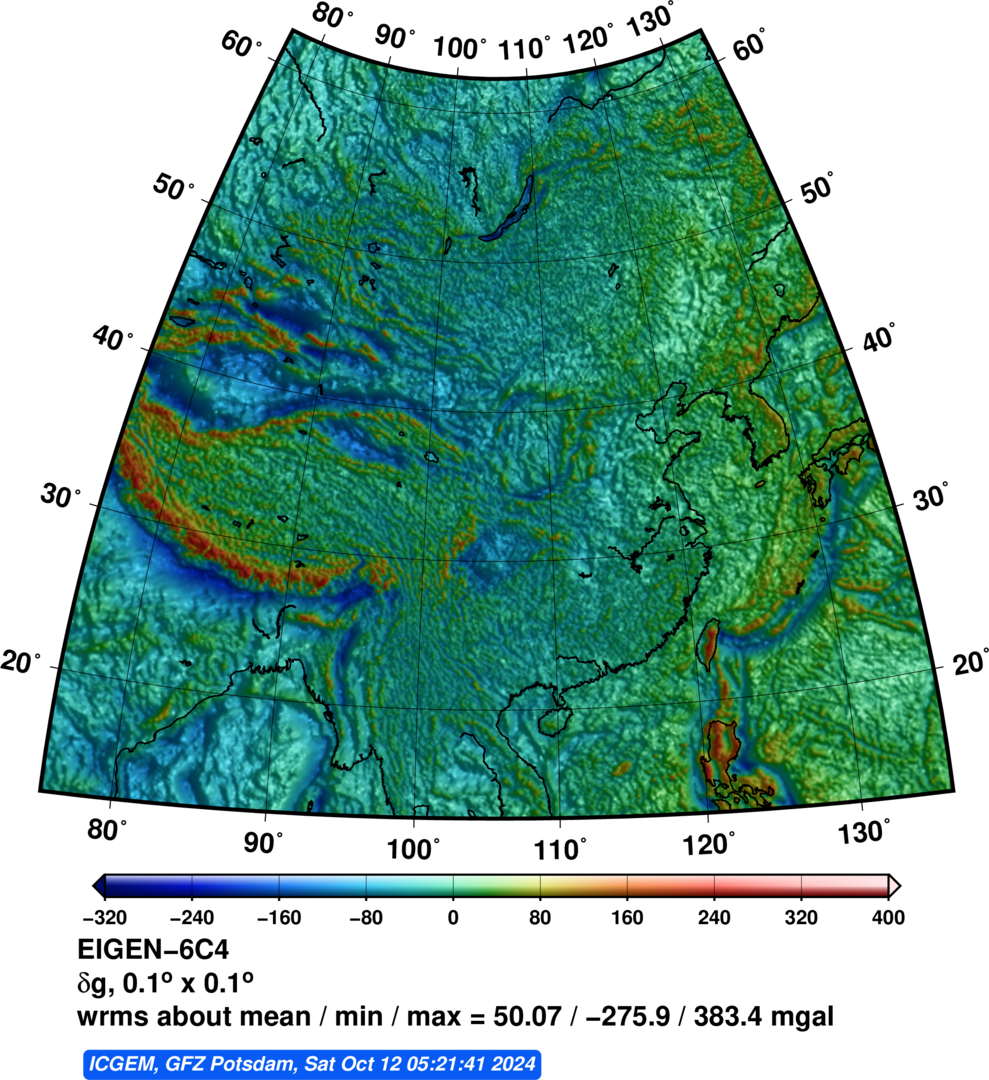
\includegraphics[width=0.91\textwidth]{figure/Grid Calculation results for gravity_disturbance of EIGEN-6C4.png}
            \end{minipage}
      }
      \captionsetup{font={footnotesize}}
      \caption{\label{fig:model_ICGEM}利用球谐模型提取重力扰动值\upcite{ince2019icgem}}
\end{figure}


在球坐标系下,重力扰动势可以表示为:
\begin{equation}
      T = \frac{GM}{r}\sum_{n=2}^{N}{\left( \frac{R_e}{r}\right)^n\sum_{m=0}^{n}(\bar{C}_{nm}^{\ast}\cos{m\lambda} + \bar{S}_{nm}^{\ast}\sin{m\lambda})\bar{P}_{nm}(\cos \theta)} 
\end{equation}
其中$G$代表牛顿引力常数,$M$代表地球的质量,$\theta$是极坐标角,可由$\theta = \frac{\pi}{2} - L$ 计算,$\lambda$是地理经度,$R_e$是参考椭球的地球长半轴,$r$为计算点到椭球中心的矢量长度,$\bar{C}_{nm}^{\ast}$和$\bar{S}_{nm}^{\ast}$表示$n$阶和$m$阶的球谐模型的系数,$\bar{P}_{nm}(\cos \theta)$是归一化的相关勒让德函数(Legendre)。根据重力与重力势的几何关系和定义,对重力扰动势求导即可计算出垂线偏差,进而也可以求解得到水平方向的重力扰动。

正常来说,只要确定了系数$\bar{C}_{nm}^{\ast}$和$\bar{S}_{nm}^{\ast}$,就可以计算垂线偏差和重力扰动,但是在实际应用中,由于数据的全球分布相对不足,且系数众多,使得该解仅局限于截断的低次展开,仅能反映全球重力场的长波长特征。此外,由于部分地区重力数据的缺失,导致局部重力场球谐模型在缺乏高频信息的情况下精度较差。而文献\cite{hao2022relative}提出了一种基于路径重力异常补偿的新的DOV计算方法,将Vening-Meinesz 公式进行离散处理\upcite{ning1994spherical,chen1982methods,ning2006refined},解决了计算效率低下和对卫星信息依赖性的问题。

文献\cite{wang2016application}论证了高分辨率球面调和引力模型比传统引力模型更能准确地表征地球重力场。在此基础上,文献\cite{wu2016gravity}提出了两种从离线数据库中插值,直接使用球谐模型计算重力矢量的重力补偿方法,有效地降低了舒勒振荡。
相较于使用全球模型,相关人员结合实测数据,精细化了地方区域的球谐函数模型\upcite{zhu2019research,weng2020analysis},极大的提升了模型的精度,但是显而易见的是,该方法仅限于特定的区域。文献\cite{Lenyue2024}则利用球谐模型和重力数据库,研究了天文/惯性组合系统中的重力扰动补偿方法。
为了进一步提高重力补偿的实时性,文献\cite{gao2021real}提出了一种基于反向传播神经网络(back-propagation neural network (BPNN))的重力预测模型,通过将规划航区内重力扰动信息作为数据集进行训练,用于纯惯导解算的实时补偿,其效果与用球谐模型补偿相同。缺点是因为其只关注于实时地去获取补偿数值,而忽略了其补偿的具体方案,并且只适用于预先规划的区域。当然,使用不同阶次的球谐模型针对不同的地形分布可能有不一样的补偿效果\upcite{Zhuhongbao2024,zhou2018},最优阶次的选择是一个值得研究的方向。

\subsection{基于实测数据补偿}
基于实测数据补偿的方法是利用大地水准面实测重力数据的插值方法获得重力扰动,然后将重力扰动处理到INS向上延续的高度\upcite{kwon2004gravity,arora2014fast}。目前用的较多的主要有反距离加权插值法\upcite{hofmann2006physical},双线性插值法\upcite{sarzeaud2009optimal},克里金法\upcite{bishop2002gravitational}和改进的二次曲面Shepard插值法\upcite{Wu2007}等。文献\cite{zhou2016novel}使用了一种基于极限学习机(Extreme Learning Machine,ELM)的方法对重力扰动估计算法建立预测模型,然后将重力扰动补偿到惯导系统误差方程中,达到抑制惯导系统误差传播的目的。
文献\cite{zhou2016improved}基于实测的数据,提出了一种基于心智进化计算(mind evolutionary computation,MEC)、反向传播(back propagation,BP)和AdaBoost算法的神经网络模型,将INS的位置坐标代入训练好的神经网络模型中,以获得重力扰动的估计值,并将这些值补偿到INS的误差方程中。该模型能够解决传统插值方法(如最小二乘配置,LSC)无法解决的输入和输出数据之间的非线性问题,位置误差的最大值可以减少28\%。文献\cite{ZHOUXIAO2016}利用小波神经网络对格网区域内重力扰动数据进行预测,相比于反距离加权插值结果,进行重力扰动补偿后其速度误差最大减小约0.2m/s,最大位置误差减小约3000m。

\subsection{基于滤波估计补偿}
通过将SINS与其他不受重力扰动影响的导航传感器结合形成组合导航系统,以实现重力扰动分量的最优估计的补偿方法,称为滤波估计补偿。
文献\cite{yang2024autonomous}揭示了重力扰动、重力扰动率和重力扰动梯度之间的内在耦合关系,建立了能准确反映重力扰动时变特性的状态空间模型,并针对旋转惯导系统,提出了一种自主高精度重力扰动实时估计和补偿的方案,车载试验的水平定位精度优于50m。垂线偏差会对姿态引入解算误差,文献\cite{an2021method}为了解决捷联惯导动态测量的问题,利用衰减记忆卡尔曼滤波器估计DOV补偿后的姿态角,并将其作为基准与捷联惯导系统得到的姿态角进行差分,得到最终轨迹上的垂线偏差值。但是,该方法没有基于初始对准的过程对姿态误差进行研究,如果初始对准的结果不准确,可能会导致整个导航过程中误差的积累。文献\cite{stepanov2020algorithms}则基于船舶起伏模型并使用Rao-Blackwellised filter滤波器来对遗传算法的参数进行识别得到了更为精确的重力估计值。文献\cite{1020386196.nh}为减小滤波器时延引起的DOV估计误差,提出了基于模型选择的自适应延迟反馈(model-based SDF)和基于调Q的姿态观测法(Q-AOM)两种实时补偿方案。钟明飞等人通过建立包含重力扰动的惯导系统误差模型\upcite{WXDH201505008015},得到了垂向重力扰动对惯性系统的姿态影响无需考虑的结论;同时他们还利用垂线偏差数据库进行了补偿,但是效果不明显。而对加速度计施加一个噪声驱动项后,利用卡尔曼滤波技术对残余误差进行实时估计后,补偿精度有较大提升。除了对惯性导航系统参数进行补偿外,文献\cite{xiong2018analysis}分析了重力异常与惯性/卫星组合导航高度的结果影响,并将其作为一阶高斯-马尔可夫过程加入到卡尔曼滤波器的状态估计中,有效降低了重力异常对高度估计的影响,但仍可能存在其他误差源未被考虑,可能影响最终的估计精度。文献\cite{fang2013accurate}则结合直接差分法和时间序列分析的重力扰动测量方法(direct-difference-modeling method,DD-M),将该模型引入定位和定向系统(position and orientation system,POS)的卡尔曼滤波器中,以估计和补偿重力扰动,显著提高了水平姿态的精度。

\subsection{基于多源数据融合补偿}
无论是球谐模型还是实时测量,单一的测量手段都无法充分描述真实重力场信息,而通过融合不同的数据源信息可以进一步地补充重力场的细节,提高数据的可靠性\upcite{DKXB20050100F}。融合多源数据的常用方法包括统计法和解析法两类\upcite{1020160654.nh},其中统计法常用最小二乘配置法,解析法则是借助球谐函数融合重力异常\upcite{kern2003analysis,2009059209.nh},利用局部重力数据的残差数据修改球谐函数系数,在迭代过程中逐步融合实测数据,常用的有双线性插值法,克立格法,径向基函数法等。为了抑制协方差矩阵小奇异值放大噪声对配置解的污染,黄谟涛在最小二乘配置中将Tikhonov正则化方法引入\upcite{HYCH201303004},提高了配置解的精度和稳定性。文献\cite{LUOKAIXIN2023}提出了多源重力数据融合算法(Multi-source gravity data fusion algorithm, MSGDFA),通过相关处理,对由零偏导致的误差进行消除。在此基础上,作者又增加了预测模型,以提高算法的实时性。文献\cite{1022810006.nh}针对水下传感器多样性的特点,提出了水下重力测量的多源数据融合的方法,并研究了基于SINS/DVL/USBL/DG的集中式卡尔曼滤波方法,获得了较高精度的水下重力数据。由于径向基函数在空间域和频率域表现出较好的局部化特性,可以融合多源重力数据,且解算效率高于最小二乘配置法\upcite{wittwer2009regional},很多学者使用该方法建立全球或局部重力场模型\upcite{bentel2013different,bentel2016combining,pham2009solutions,klees2008data,CHXB201609003,DQWX201704009,mahbuby2017local,tenzer2008choice}。

\subsection{基于频段信息补偿}
对于低速运行的载体来说,水平重力扰动的高频信号对惯性导航的定位误差影响较大,因此深入分析重力扰动的频率特征与惯性导航系统的误差特征之间的关系,可以更好的对重力扰动进行补偿。Jekeli通过空间和频域的协方差分析,提出了在相对稳定的无补偿陀螺漂移条件下,可以不借助外界姿态更新的情况下估计短波重力矢量\upcite{jekeli1994airborne}。文献\cite{Zhuhongbao2024}提出,水平通道对重力扰动的高频信号具有低通滤波的作用,认为补偿频段在截止频率的区间内不会损失精度。在利用球谐模型的基础上,文献\cite{Liuyuxin2023}和文献\cite{dai2014improved}提出了一种球谐模型补偿与状态估计补偿相互结合的高精度重力扰动补偿方法,对长波采取球谐模型补偿,而利用马尔可夫模型对中短波重力扰动分量进行状态估计,整体上相比单一的补偿效果更好。文献\cite{Zhangpanpan23}则利用剩余地形模型(Residual Terrian Model,RTM)技术恢复高频重力场信号,弥补高阶重力场模型短波信号缺失的不足。同样,文献\cite{tenzer2010effect}认为,地形校正的平滑效果只对重力信号的高频部分有效。

\begin{figure}[h]
      \centering
      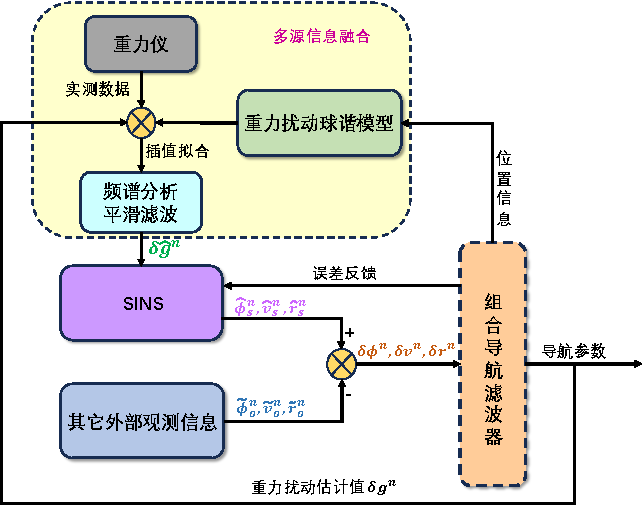
\includegraphics[width=0.55\textwidth]{figure/fig_compensation-crop.pdf}
      \captionsetup{font={footnotesize}}
      \caption{\label{fig:compensation}重力扰动补偿方案框图}
\end{figure}

图\ref{fig:compensation}为现有的重力扰动补偿方案的流程框图。除了以上具体的方法外,相关研究人员针对不同场景和地理环境提出了相应的补偿方法,比如文献\cite{LIQIAN2022}研究的在极区环境下利用其对极区横坐标系捷联惯性导航系统解算实现重力扰动补偿。
\section{总结与展望}
海洋是人类不断探索大自然的奥秘的重要一环,而现有情况下,惯性导航系统凭借其自主无源的优势,在水下导航方面有很大的发展前景。但是,同样又受制于海洋环境的特殊性与现有的器件工艺水平,在水下能够真正实现无源辅助惯性导航可能的是凭借地球自身的重力场特性。现有的测量仪器中,捷联式重力仪具有体积小、操作便捷、易于集成在各种载体上使用等优点,已经成熟地应用于航空、地面和船载等不同场景。随着惯性器件精度不断提升,器件误差的量级将会小于重力扰动的量级,对于高精度惯导来说,补偿重力扰动对于抑制其误差的发散具有一定的作用。但是,目前大部分的应用重力补偿方法是基于球谐模型和重力数据库的补偿方法,然而使用该方法对于设备硬件的计算或者存储成本是一个很大的挑战,在条件不足的情况下可能无法满足现有的实时补偿,更多往往应用于导航后处理;而利用实测数据或者滤波估计算法进行补偿,却往往因为其精度与处理的复杂性等原因而得不到有效地应用。更重要的是,目前现有的补偿策略方法相对比较单一,因此,在本篇文章的基础上,作者提出以下几点意见建议:

1、在现有的重力测量基本原理上,对各种误差源进行分析建模,根据实际情况采用不同的滤波算法实现多信息源融合,进一步丰富重力测量的数据;

2、建议在完善重力扰动对惯导系统的影响机理的分析基础上,建立实时有效的补偿评估方法,明确不同的状态性能效果情况下采取何种补偿方法才更为有效,在制定相应的指标精度需求上,完善补偿流程;

3、加快推进海洋重力场的测量工作,特别是远海、深海等复杂海域,为下一步的重力修正工作提供更精确的重力场数据模型;

4、加快研制更高精度的国产化重力仪,推广其商业价值与应用价值,同时发展一套综合的、智能化的重力辅助惯性导航的系统软件,以打破国外的技术垄断。

\newpage
% \subsection{致谢}
% 感谢博客园博主\href{https://www.cnblogs.com/huangliu1111/p/13625826.html}{@望舒}提供的部分代码参考,开源促进世界进步!
% \subsection{联系作者}
% 作者QQ邮箱\href{https://wx.mail.qq.com/?cancel_login=true&from=get_ticket_fail}{1141470651@qq.com},欢迎进行讨论交流$(>\text{w}<)$,good luck!。

% \subsection{写作心得}
% 哈哈哈哈,没有么好写的心得,加油吧,一起!
% 加油加油!!!
% 哈哈哈,加油加油!!!
% 略略略,小飞棍来咯!我要睡觉!
% 我TM莱纳!
\bibliography{sample}

\end{document}